% Options for packages loaded elsewhere
% Options for packages loaded elsewhere
\PassOptionsToPackage{unicode}{hyperref}
\PassOptionsToPackage{hyphens}{url}
\PassOptionsToPackage{dvipsnames,svgnames,x11names}{xcolor}
%
\documentclass[
  letterpaper,
  DIV=11,
  numbers=noendperiod]{scrartcl}
\usepackage{xcolor}
\usepackage{amsmath,amssymb}
\setcounter{secnumdepth}{-\maxdimen} % remove section numbering
\usepackage{iftex}
\ifPDFTeX
  \usepackage[T1]{fontenc}
  \usepackage[utf8]{inputenc}
  \usepackage{textcomp} % provide euro and other symbols
\else % if luatex or xetex
  \usepackage{unicode-math} % this also loads fontspec
  \defaultfontfeatures{Scale=MatchLowercase}
  \defaultfontfeatures[\rmfamily]{Ligatures=TeX,Scale=1}
\fi
\usepackage{lmodern}
\ifPDFTeX\else
  % xetex/luatex font selection
\fi
% Use upquote if available, for straight quotes in verbatim environments
\IfFileExists{upquote.sty}{\usepackage{upquote}}{}
\IfFileExists{microtype.sty}{% use microtype if available
  \usepackage[]{microtype}
  \UseMicrotypeSet[protrusion]{basicmath} % disable protrusion for tt fonts
}{}
\makeatletter
\@ifundefined{KOMAClassName}{% if non-KOMA class
  \IfFileExists{parskip.sty}{%
    \usepackage{parskip}
  }{% else
    \setlength{\parindent}{0pt}
    \setlength{\parskip}{6pt plus 2pt minus 1pt}}
}{% if KOMA class
  \KOMAoptions{parskip=half}}
\makeatother
% Make \paragraph and \subparagraph free-standing
\makeatletter
\ifx\paragraph\undefined\else
  \let\oldparagraph\paragraph
  \renewcommand{\paragraph}{
    \@ifstar
      \xxxParagraphStar
      \xxxParagraphNoStar
  }
  \newcommand{\xxxParagraphStar}[1]{\oldparagraph*{#1}\mbox{}}
  \newcommand{\xxxParagraphNoStar}[1]{\oldparagraph{#1}\mbox{}}
\fi
\ifx\subparagraph\undefined\else
  \let\oldsubparagraph\subparagraph
  \renewcommand{\subparagraph}{
    \@ifstar
      \xxxSubParagraphStar
      \xxxSubParagraphNoStar
  }
  \newcommand{\xxxSubParagraphStar}[1]{\oldsubparagraph*{#1}\mbox{}}
  \newcommand{\xxxSubParagraphNoStar}[1]{\oldsubparagraph{#1}\mbox{}}
\fi
\makeatother

\usepackage{color}
\usepackage{fancyvrb}
\newcommand{\VerbBar}{|}
\newcommand{\VERB}{\Verb[commandchars=\\\{\}]}
\DefineVerbatimEnvironment{Highlighting}{Verbatim}{commandchars=\\\{\}}
% Add ',fontsize=\small' for more characters per line
\usepackage{framed}
\definecolor{shadecolor}{RGB}{241,243,245}
\newenvironment{Shaded}{\begin{snugshade}}{\end{snugshade}}
\newcommand{\AlertTok}[1]{\textcolor[rgb]{0.68,0.00,0.00}{#1}}
\newcommand{\AnnotationTok}[1]{\textcolor[rgb]{0.37,0.37,0.37}{#1}}
\newcommand{\AttributeTok}[1]{\textcolor[rgb]{0.40,0.45,0.13}{#1}}
\newcommand{\BaseNTok}[1]{\textcolor[rgb]{0.68,0.00,0.00}{#1}}
\newcommand{\BuiltInTok}[1]{\textcolor[rgb]{0.00,0.23,0.31}{#1}}
\newcommand{\CharTok}[1]{\textcolor[rgb]{0.13,0.47,0.30}{#1}}
\newcommand{\CommentTok}[1]{\textcolor[rgb]{0.37,0.37,0.37}{#1}}
\newcommand{\CommentVarTok}[1]{\textcolor[rgb]{0.37,0.37,0.37}{\textit{#1}}}
\newcommand{\ConstantTok}[1]{\textcolor[rgb]{0.56,0.35,0.01}{#1}}
\newcommand{\ControlFlowTok}[1]{\textcolor[rgb]{0.00,0.23,0.31}{\textbf{#1}}}
\newcommand{\DataTypeTok}[1]{\textcolor[rgb]{0.68,0.00,0.00}{#1}}
\newcommand{\DecValTok}[1]{\textcolor[rgb]{0.68,0.00,0.00}{#1}}
\newcommand{\DocumentationTok}[1]{\textcolor[rgb]{0.37,0.37,0.37}{\textit{#1}}}
\newcommand{\ErrorTok}[1]{\textcolor[rgb]{0.68,0.00,0.00}{#1}}
\newcommand{\ExtensionTok}[1]{\textcolor[rgb]{0.00,0.23,0.31}{#1}}
\newcommand{\FloatTok}[1]{\textcolor[rgb]{0.68,0.00,0.00}{#1}}
\newcommand{\FunctionTok}[1]{\textcolor[rgb]{0.28,0.35,0.67}{#1}}
\newcommand{\ImportTok}[1]{\textcolor[rgb]{0.00,0.46,0.62}{#1}}
\newcommand{\InformationTok}[1]{\textcolor[rgb]{0.37,0.37,0.37}{#1}}
\newcommand{\KeywordTok}[1]{\textcolor[rgb]{0.00,0.23,0.31}{\textbf{#1}}}
\newcommand{\NormalTok}[1]{\textcolor[rgb]{0.00,0.23,0.31}{#1}}
\newcommand{\OperatorTok}[1]{\textcolor[rgb]{0.37,0.37,0.37}{#1}}
\newcommand{\OtherTok}[1]{\textcolor[rgb]{0.00,0.23,0.31}{#1}}
\newcommand{\PreprocessorTok}[1]{\textcolor[rgb]{0.68,0.00,0.00}{#1}}
\newcommand{\RegionMarkerTok}[1]{\textcolor[rgb]{0.00,0.23,0.31}{#1}}
\newcommand{\SpecialCharTok}[1]{\textcolor[rgb]{0.37,0.37,0.37}{#1}}
\newcommand{\SpecialStringTok}[1]{\textcolor[rgb]{0.13,0.47,0.30}{#1}}
\newcommand{\StringTok}[1]{\textcolor[rgb]{0.13,0.47,0.30}{#1}}
\newcommand{\VariableTok}[1]{\textcolor[rgb]{0.07,0.07,0.07}{#1}}
\newcommand{\VerbatimStringTok}[1]{\textcolor[rgb]{0.13,0.47,0.30}{#1}}
\newcommand{\WarningTok}[1]{\textcolor[rgb]{0.37,0.37,0.37}{\textit{#1}}}

\usepackage{longtable,booktabs,array}
\newcounter{none} % for unnumbered tables
\usepackage{calc} % for calculating minipage widths
% Correct order of tables after \paragraph or \subparagraph
\usepackage{etoolbox}
\makeatletter
\patchcmd\longtable{\par}{\if@noskipsec\mbox{}\fi\par}{}{}
\makeatother
% Allow footnotes in longtable head/foot
\IfFileExists{footnotehyper.sty}{\usepackage{footnotehyper}}{\usepackage{footnote}}
\makesavenoteenv{longtable}
\usepackage{graphicx}
\makeatletter
\newsavebox\pandoc@box
\newcommand*\pandocbounded[1]{% scales image to fit in text height/width
  \sbox\pandoc@box{#1}%
  \Gscale@div\@tempa{\textheight}{\dimexpr\ht\pandoc@box+\dp\pandoc@box\relax}%
  \Gscale@div\@tempb{\linewidth}{\wd\pandoc@box}%
  \ifdim\@tempb\p@<\@tempa\p@\let\@tempa\@tempb\fi% select the smaller of both
  \ifdim\@tempa\p@<\p@\scalebox{\@tempa}{\usebox\pandoc@box}%
  \else\usebox{\pandoc@box}%
  \fi%
}
% Set default figure placement to htbp
\def\fps@figure{htbp}
\makeatother





\setlength{\emergencystretch}{3em} % prevent overfull lines

\providecommand{\tightlist}{%
  \setlength{\itemsep}{0pt}\setlength{\parskip}{0pt}}



 


\KOMAoption{captions}{tableheading}
\makeatletter
\@ifpackageloaded{tcolorbox}{}{\usepackage[skins,breakable]{tcolorbox}}
\@ifpackageloaded{fontawesome5}{}{\usepackage{fontawesome5}}
\definecolor{quarto-callout-color}{HTML}{909090}
\definecolor{quarto-callout-note-color}{HTML}{0758E5}
\definecolor{quarto-callout-important-color}{HTML}{CC1914}
\definecolor{quarto-callout-warning-color}{HTML}{EB9113}
\definecolor{quarto-callout-tip-color}{HTML}{00A047}
\definecolor{quarto-callout-caution-color}{HTML}{FC5300}
\definecolor{quarto-callout-color-frame}{HTML}{acacac}
\definecolor{quarto-callout-note-color-frame}{HTML}{4582ec}
\definecolor{quarto-callout-important-color-frame}{HTML}{d9534f}
\definecolor{quarto-callout-warning-color-frame}{HTML}{f0ad4e}
\definecolor{quarto-callout-tip-color-frame}{HTML}{02b875}
\definecolor{quarto-callout-caution-color-frame}{HTML}{fd7e14}
\makeatother
\makeatletter
\@ifpackageloaded{caption}{}{\usepackage{caption}}
\AtBeginDocument{%
\ifdefined\contentsname
  \renewcommand*\contentsname{Table of contents}
\else
  \newcommand\contentsname{Table of contents}
\fi
\ifdefined\listfigurename
  \renewcommand*\listfigurename{List of Figures}
\else
  \newcommand\listfigurename{List of Figures}
\fi
\ifdefined\listtablename
  \renewcommand*\listtablename{List of Tables}
\else
  \newcommand\listtablename{List of Tables}
\fi
\ifdefined\figurename
  \renewcommand*\figurename{Figure}
\else
  \newcommand\figurename{Figure}
\fi
\ifdefined\tablename
  \renewcommand*\tablename{Table}
\else
  \newcommand\tablename{Table}
\fi
}
\@ifpackageloaded{float}{}{\usepackage{float}}
\floatstyle{ruled}
\@ifundefined{c@chapter}{\newfloat{codelisting}{h}{lop}}{\newfloat{codelisting}{h}{lop}[chapter]}
\floatname{codelisting}{Listing}
\newcommand*\listoflistings{\listof{codelisting}{List of Listings}}
\makeatother
\makeatletter
\makeatother
\makeatletter
\@ifpackageloaded{caption}{}{\usepackage{caption}}
\@ifpackageloaded{subcaption}{}{\usepackage{subcaption}}
\makeatother
\makeatletter
\@ifpackageloaded{tikz}{}{\usepackage{tikz}}
\makeatother
        \newcommand*\circled[1]{\tikz[baseline=(char.base)]{
          \node[shape=circle,draw,inner sep=1pt] (char) {{\scriptsize#1}};}}  
                  
\usepackage{bookmark}
\IfFileExists{xurl.sty}{\usepackage{xurl}}{} % add URL line breaks if available
\urlstyle{same}
\hypersetup{
  pdftitle={Slide design: chunks{,} bullets or paragraphs?},
  pdfauthor={Mike and Rieke},
  colorlinks=true,
  linkcolor={blue},
  filecolor={Maroon},
  citecolor={Blue},
  urlcolor={Blue},
  pdfcreator={LaTeX via pandoc}}


\title{Slide design: chunks, bullets or paragraphs?}
\author{Mike and Rieke}
\date{2026-06-16}
\begin{document}
\maketitle

\renewcommand*\contentsname{Table of contents}
{
\setcounter{tocdepth}{3}
\tableofcontents
}

\begin{Shaded}
\begin{Highlighting}[]
\ImportTok{import}\NormalTok{ os}
\ImportTok{import}\NormalTok{ glob}
\ImportTok{import}\NormalTok{ pandas }\ImportTok{as}\NormalTok{ pd}
\ImportTok{import}\NormalTok{ re}
\ImportTok{import}\NormalTok{ random}
\ImportTok{import}\NormalTok{ numpy }\ImportTok{as}\NormalTok{ np}
\ImportTok{import}\NormalTok{ scipy.stats }\ImportTok{as}\NormalTok{ stats}
\ImportTok{import}\NormalTok{ statsmodels.stats.multicomp }\ImportTok{as}\NormalTok{ mc}
\ImportTok{import}\NormalTok{ statsmodels.formula.api }\ImportTok{as}\NormalTok{ smf}
\ImportTok{from}\NormalTok{ statsmodels.stats.anova }\ImportTok{import}\NormalTok{ anova\_lm}
\ImportTok{from}\NormalTok{ plotnine }\ImportTok{import} \OperatorTok{*} 
\ImportTok{from}\NormalTok{ IPython.display }\ImportTok{import}\NormalTok{ Markdown, display}
\ImportTok{from}\NormalTok{ tabulate }\ImportTok{import}\NormalTok{ tabulate}
\end{Highlighting}
\end{Shaded}

\section{Functions}\label{functions}

\begin{Shaded}
\begin{Highlighting}[]
\CommentTok{\# Function to read CSV and add condition column}
\KeywordTok{def}\NormalTok{ read\_csv\_with\_condition(file\_path):}
\NormalTok{    df }\OperatorTok{=}\NormalTok{ pd.read\_csv(file\_path, header}\OperatorTok{=}\NormalTok{[}\DecValTok{0}\NormalTok{], skiprows }\OperatorTok{=}\NormalTok{ [}\DecValTok{1}\NormalTok{])}
\NormalTok{    condition\_name }\OperatorTok{=}\NormalTok{ os.path.splitext(os.path.basename(file\_path))[}\DecValTok{0}\NormalTok{].replace(study\_name}\OperatorTok{+}\StringTok{"{-}"}\NormalTok{, }\StringTok{""}\NormalTok{)  }\CommentTok{\# Get filename without extension and remove the study round}
\NormalTok{    df[}\StringTok{\textquotesingle{}condition\textquotesingle{}}\NormalTok{] }\OperatorTok{=}\NormalTok{ condition\_name  }\CommentTok{\# Add condition column}
\NormalTok{    df[}\StringTok{\textquotesingle{}conditionLength\textquotesingle{}}\NormalTok{] }\OperatorTok{=} \BuiltInTok{int}\NormalTok{(condition\_name.split(}\StringTok{\textquotesingle{}{-}\textquotesingle{}}\NormalTok{)[}\DecValTok{0}\NormalTok{])}
\NormalTok{    df[}\StringTok{\textquotesingle{}conditionType\textquotesingle{}}\NormalTok{] }\OperatorTok{=}\NormalTok{ condition\_name.split(}\StringTok{\textquotesingle{}{-}\textquotesingle{}}\NormalTok{)[}\DecValTok{1}\NormalTok{]}
    \ControlFlowTok{return}\NormalTok{ df, condition\_name}

\CommentTok{\# Function to combine headers}
\KeywordTok{def}\NormalTok{ combine\_headers(df):}
\NormalTok{    df.columns }\OperatorTok{=}\NormalTok{ [}\StringTok{\textquotesingle{} \textquotesingle{}}\NormalTok{.join(col).strip() }\ControlFlowTok{for}\NormalTok{ col }\KeywordTok{in}\NormalTok{ df.columns.values]}
    \ControlFlowTok{return}\NormalTok{ df}

\CommentTok{\# Clean remaining column names}
\KeywordTok{def}\NormalTok{ clean\_column\_names(columns):}
\NormalTok{    cleaned\_columns }\OperatorTok{=}\NormalTok{ []}
    \ControlFlowTok{for}\NormalTok{ col }\KeywordTok{in}\NormalTok{ columns:}
\NormalTok{        col }\OperatorTok{=}\NormalTok{ re.sub(}\VerbatimStringTok{r\textquotesingle{}}\DecValTok{\textbackslash{}b}\VerbatimStringTok{response}\DecValTok{\textbackslash{}b}\VerbatimStringTok{\textquotesingle{}}\NormalTok{, }\StringTok{\textquotesingle{}\textquotesingle{}}\NormalTok{, col, flags}\OperatorTok{=}\NormalTok{re.IGNORECASE)}
\NormalTok{        col }\OperatorTok{=}\NormalTok{ re.sub(}\VerbatimStringTok{r\textquotesingle{}}\PreprocessorTok{[\^{}a{-}zA{-}Z0{-}9]}\VerbatimStringTok{\textquotesingle{}}\NormalTok{, }\StringTok{\textquotesingle{}\_\textquotesingle{}}\NormalTok{, col).lower()}
\NormalTok{        col }\OperatorTok{=}\NormalTok{ col.strip(}\StringTok{\textquotesingle{}\_\textquotesingle{}}\NormalTok{)}
\NormalTok{        cleaned\_columns.append(col)}
    \ControlFlowTok{return}\NormalTok{ cleaned\_columns}
  
\CommentTok{\# Function to check answers and add correctness columns}
\KeywordTok{def}\NormalTok{ add\_correctness\_columns(df, answer\_map):}
    \ControlFlowTok{for}\NormalTok{ column, correct\_answer }\KeywordTok{in}\NormalTok{ answer\_map.items():}
        \ControlFlowTok{if}\NormalTok{ column }\KeywordTok{in}\NormalTok{ df.columns:}
\NormalTok{            df[column] }\OperatorTok{=}\NormalTok{ df[column].fillna(}\StringTok{""}\NormalTok{)}
            \CommentTok{\# Create a new column with 1 if correct, 0 if incorrect}
\NormalTok{            df[}\SpecialStringTok{f\textquotesingle{}}\SpecialCharTok{\{}\NormalTok{column}\SpecialCharTok{\}}\SpecialStringTok{\_correct\textquotesingle{}}\NormalTok{] }\OperatorTok{=}\NormalTok{ np.where(df[column].}\BuiltInTok{str}\NormalTok{.strip().}\BuiltInTok{str}\NormalTok{.lower() }\OperatorTok{==}\NormalTok{ correct\_answer.lower(), }\DecValTok{1}\NormalTok{, }\DecValTok{0}\NormalTok{)}
    \ControlFlowTok{return}\NormalTok{ df}

\CommentTok{\# Function to add a total correct column for each participant}
\KeywordTok{def}\NormalTok{ add\_total\_correct\_column(df):}
    \CommentTok{\# Identify all correctness columns (columns ending with \textquotesingle{}\_correct\textquotesingle{})}
\NormalTok{    correctness\_columns }\OperatorTok{=}\NormalTok{ [col }\ControlFlowTok{for}\NormalTok{ col }\KeywordTok{in}\NormalTok{ df.columns }\ControlFlowTok{if}\NormalTok{ col.endswith(}\StringTok{\textquotesingle{}\_correct\textquotesingle{}}\NormalTok{)]}
    \CommentTok{\# Sum the correctness columns to create the total correct column}
\NormalTok{    df[}\StringTok{\textquotesingle{}total\_correct\textquotesingle{}}\NormalTok{] }\OperatorTok{=}\NormalTok{ df[correctness\_columns].}\BuiltInTok{sum}\NormalTok{(axis}\OperatorTok{=}\DecValTok{1}\NormalTok{)}
    \ControlFlowTok{return}\NormalTok{ df}
  
\CommentTok{\# Function to merge the answers to a single question into one column}
\KeywordTok{def}\NormalTok{ merge\_columnes(df, column\_name, number\_of\_columns):}
  \CommentTok{\#number\_of\_columns needs to be the total number, not just the ones that are to be merged}
\NormalTok{  loc\_index }\OperatorTok{=}\NormalTok{ df.columns.get\_loc(column\_name)}
\NormalTok{  df[column\_name] }\OperatorTok{=}\NormalTok{ df.iloc[:, loc\_index:loc\_index}\OperatorTok{+}\NormalTok{number\_of\_columns].bfill(axis}\OperatorTok{=}\DecValTok{1}\NormalTok{).iloc[:, }\DecValTok{0}\NormalTok{]}
\NormalTok{  df.drop(df.columns[loc\_index}\OperatorTok{+}\DecValTok{1}\NormalTok{:loc\_index}\OperatorTok{+}\NormalTok{number\_of\_columns], axis}\OperatorTok{=}\DecValTok{1}\NormalTok{, inplace}\OperatorTok{=}\VariableTok{True}\NormalTok{)}
  \ControlFlowTok{return}\NormalTok{ df}

\CommentTok{\#function to calculate and print U{-}test}
\KeywordTok{def}\NormalTok{ utest(cond1, cond2):}
\NormalTok{  results }\OperatorTok{=}\NormalTok{ \{\}}

  \ControlFlowTok{for}\NormalTok{ column }\KeywordTok{in}\NormalTok{ test\_columns:}
\NormalTok{    df\_combined\_dropna }\OperatorTok{=}\NormalTok{ df\_combined.dropna(subset }\OperatorTok{=}\NormalTok{ [column], inplace}\OperatorTok{=}\VariableTok{False}\NormalTok{)}
\NormalTok{    U1, p }\OperatorTok{=}\NormalTok{ stats.mannwhitneyu(df\_combined\_dropna[column][df\_combined\_dropna[}\StringTok{\textquotesingle{}condition\textquotesingle{}}\NormalTok{] }\OperatorTok{==}\NormalTok{ cond1],}
\NormalTok{                df\_combined\_dropna[column][df\_combined\_dropna[}\StringTok{\textquotesingle{}condition\textquotesingle{}}\NormalTok{] }\OperatorTok{==}\NormalTok{ cond2], method}\OperatorTok{=}\StringTok{"exact"}\NormalTok{)}
\NormalTok{    results[column] }\OperatorTok{=}\NormalTok{ \{}\StringTok{\textquotesingle{}U1\_stat\textquotesingle{}}\NormalTok{: U1, }\StringTok{\textquotesingle{}p\_value\textquotesingle{}}\NormalTok{: p\}}
  
\NormalTok{  df }\OperatorTok{=}\NormalTok{ pd.DataFrame.from\_dict(results, orient }\OperatorTok{=} \StringTok{"index"}\NormalTok{)}
\NormalTok{  df.index }\OperatorTok{=}\NormalTok{ test\_column\_names}
\NormalTok{  Markdown(tabulate(df, headers }\OperatorTok{=}\NormalTok{ [}\StringTok{"U1 statistic"}\NormalTok{, }\StringTok{"p{-}value"}\NormalTok{]))}

\NormalTok{  display(Markdown(df.to\_markdown()))}
\end{Highlighting}
\end{Shaded}

\section{Load data}\label{load-data}

\protect\phantomsection\label{annotated-cell-3}%
\begin{Shaded}
\begin{Highlighting}[]
\NormalTok{study\_name }\OperatorTok{=} \StringTok{"pg"}
\NormalTok{file\_list }\OperatorTok{=}\NormalTok{ glob.glob(os.path.join(os.getcwd(), }\StringTok{"data/2025{-}10{-}19\_SurveyData"}\NormalTok{, study\_name}\OperatorTok{+}\StringTok{"*.csv"}\NormalTok{)) }\hspace*{\fill}\NormalTok{\circled{1}}

\ControlFlowTok{for}\NormalTok{ f }\KeywordTok{in}\NormalTok{ file\_list:}
    \BuiltInTok{print}\NormalTok{(os.path.basename(f))}

\NormalTok{df\_combined }\OperatorTok{=}\NormalTok{ pd.DataFrame(\{\})}
\NormalTok{condition\_list }\OperatorTok{=}\NormalTok{ []}

\ControlFlowTok{for}\NormalTok{ i }\KeywordTok{in} \BuiltInTok{range}\NormalTok{(}\BuiltInTok{len}\NormalTok{(file\_list)):}
\NormalTok{  new\_file, conditionname }\OperatorTok{=}\NormalTok{ read\_csv\_with\_condition(file\_list[i]) }\hspace*{\fill}\NormalTok{\circled{2}}
\NormalTok{  df\_combined }\OperatorTok{=}\NormalTok{ pd.concat([df\_combined, new\_file], ignore\_index }\OperatorTok{=} \VariableTok{True}\NormalTok{) }\hspace*{\fill}\NormalTok{\circled{3}}
\NormalTok{  condition\_list.append(conditionname) }\hspace*{\fill}\NormalTok{\circled{4}}

\NormalTok{df\_combined }\OperatorTok{=}\NormalTok{ df\_combined.convert\_dtypes() }\hspace*{\fill}\NormalTok{\circled{5}}
\end{Highlighting}
\end{Shaded}

\begin{description}
\tightlist
\item[\circled{1}]
Get list of all files for this study round.
\item[\circled{2}]
Read the files.
\item[\circled{3}]
Create dataframe with all the data.
\item[\circled{4}]
Create a list of all studied conditions
\item[\circled{5}]
To make processing easier, we convert the data types for the whole data
frame right away.
\end{description}

\begin{verbatim}
pg-100-bullets.csv
pg-100-chunks.csv
pg-100-para.csv
pg-30-bullets.csv
pg-30-chunks.csv
pg-30-para.csv
pg-50-bullets.csv
pg-50-chunks.csv
pg-50-para.csv
\end{verbatim}

\section{Clean data}\label{clean-data}

Rename columns to make processing easier

\begin{Shaded}
\begin{Highlighting}[]
\NormalTok{rename\_map }\OperatorTok{=}\NormalTok{ \{}
    \StringTok{\textquotesingle{}Please rate these slides I found the slides to be attractive.\textquotesingle{}}\NormalTok{: }
      \StringTok{\textquotesingle{}slides\_attractive\textquotesingle{}}\NormalTok{,}
    \StringTok{\textquotesingle{}In what year did the Tasmanian Tiger go extinct?\textquotesingle{}}\NormalTok{: }
      \StringTok{\textquotesingle{}tiger\_extinct\_year\textquotesingle{}}\NormalTok{,}
    \StringTok{\textquotesingle{}What kind of animal would the Tasmanian Tiger be classified as?\textquotesingle{}}\NormalTok{: }
      \StringTok{\textquotesingle{}tiger\_classified\textquotesingle{}}\NormalTok{,}
    \StringTok{"What were the primary causes of the Tasmanian Tiger\textquotesingle{}s extinction?"}\NormalTok{: }
      \StringTok{\textquotesingle{}tiger\_extinct\_why\textquotesingle{}}\NormalTok{,}
    \StringTok{\textquotesingle{}Why are exoplanets important to the search for life beyond Earth?\textquotesingle{}}\NormalTok{: }
      \StringTok{\textquotesingle{}why\_exoplanets\_important\textquotesingle{}}\NormalTok{,}
    \StringTok{\textquotesingle{}Why do scientists prioritize Earth{-}like planets in their search for life?\textquotesingle{}}\NormalTok{: }
      \StringTok{\textquotesingle{}why\_prioritize\_earthlike\_planets\textquotesingle{}}\NormalTok{,}
    \StringTok{\textquotesingle{}Exoplanets were discovered in which year?\textquotesingle{}}\NormalTok{: }
      \StringTok{\textquotesingle{}exoplanets\_discovered\_year\textquotesingle{}}\NormalTok{,}
    \StringTok{\textquotesingle{}What do AI automation and chatbots primarily help reduce in customer service?\textquotesingle{}}\NormalTok{: }
      \StringTok{\textquotesingle{}what\_chatbots\_reduce\textquotesingle{}}\NormalTok{,}
    \StringTok{\textquotesingle{}What role do CRM systems play in customer service?\textquotesingle{}}\NormalTok{: }
      \StringTok{\textquotesingle{}what\_role\_crms\_play\textquotesingle{}}\NormalTok{,}
    \StringTok{\textquotesingle{}What is the relationship between 24/7 support and overall efficiency in customer service?\textquotesingle{}}\NormalTok{: }
      \StringTok{\textquotesingle{}relationship\_24\_7\_efficiency\textquotesingle{}}\NormalTok{,}
    \StringTok{\textquotesingle{}Please rate these slides\textquotesingle{}}\NormalTok{: }
      \StringTok{\textquotesingle{}slides\_attractive\textquotesingle{}}\NormalTok{,}
    \StringTok{\textquotesingle{}Unnamed: 19\textquotesingle{}}\NormalTok{: }
      \StringTok{\textquotesingle{}slides\_clean\_simple\textquotesingle{}}\NormalTok{,}
    \StringTok{\textquotesingle{}In reviewing the slides, I invested:\textquotesingle{}}\NormalTok{: }
      \StringTok{\textquotesingle{}cognitive\_load\textquotesingle{}}\NormalTok{,}
    \StringTok{\textquotesingle{}What is the highest level of education you have completed?  \textquotesingle{}}\NormalTok{: }
      \StringTok{\textquotesingle{}highest\_education\textquotesingle{}}\NormalTok{,}
    \StringTok{\textquotesingle{}How often do you create presentations with slides (for yourself or others)?\textquotesingle{}}\NormalTok{: }
      \StringTok{\textquotesingle{}creation\_frequency\textquotesingle{}}\NormalTok{,}
    \StringTok{"Enter your email. This is just to make sure we only count you once. We won\textquotesingle{}t spam you."}\NormalTok{: }\StringTok{\textquotesingle{}email\textquotesingle{}}
\NormalTok{\}}
\NormalTok{df\_combined.rename(columns}\OperatorTok{=}\NormalTok{rename\_map, inplace}\OperatorTok{=}\VariableTok{True}\NormalTok{)}

\NormalTok{df\_combined.columns }\OperatorTok{=}\NormalTok{ clean\_column\_names(df\_combined.columns)}
\end{Highlighting}
\end{Shaded}

Remove empty columns

\begin{Shaded}
\begin{Highlighting}[]
\NormalTok{blank\_columns }\OperatorTok{=}\NormalTok{ [col }\ControlFlowTok{for}\NormalTok{ col }\KeywordTok{in}\NormalTok{ df\_combined.columns }\ControlFlowTok{if}\NormalTok{ df\_combined[col].isna().}\BuiltInTok{all}\NormalTok{()]}
\NormalTok{df\_combined.drop(columns}\OperatorTok{=}\NormalTok{blank\_columns, inplace}\OperatorTok{=}\VariableTok{True}\NormalTok{)}
\end{Highlighting}
\end{Shaded}

Remove duplicates

\begin{Shaded}
\begin{Highlighting}[]
\CommentTok{\#https://stackoverflow.com/questions/23512339/drop{-}duplicates{-}while{-}preserving{-}nans{-}in{-}pandas}
\NormalTok{df\_combined }\OperatorTok{=}\NormalTok{ df\_combined[(}\OperatorTok{\textasciitilde{}}\NormalTok{df\_combined.duplicated()) ]}
\end{Highlighting}
\end{Shaded}

\section{Evaluate correctness of
answers}\label{evaluate-correctness-of-answers}

Dictionary with correct answers

\begin{Shaded}
\begin{Highlighting}[]
\NormalTok{correct\_answers }\OperatorTok{=}\NormalTok{ \{}
    \StringTok{\textquotesingle{}tiger\_extinct\_year\textquotesingle{}}\NormalTok{: }\StringTok{\textquotesingle{}1936\textquotesingle{}}\NormalTok{,}
    \StringTok{\textquotesingle{}tiger\_classified\textquotesingle{}}\NormalTok{: }\StringTok{\textquotesingle{}Marsupial\textquotesingle{}}\NormalTok{,}
    \StringTok{\textquotesingle{}tiger\_extinct\_why\textquotesingle{}}\NormalTok{: }\StringTok{\textquotesingle{}Hunting and habitat loss\textquotesingle{}}\NormalTok{,}
    \StringTok{\textquotesingle{}why\_exoplanets\_important\textquotesingle{}}\NormalTok{: }
      \StringTok{\textquotesingle{}They may be habitable and contain liquid water, and biosignatures.\textquotesingle{}}\NormalTok{,}
    \StringTok{\textquotesingle{}why\_prioritize\_earthlike\_planets\textquotesingle{}}\NormalTok{: }
      \StringTok{\textquotesingle{}They might have liquid water and biosignatures.\textquotesingle{}}\NormalTok{,}
    \StringTok{\textquotesingle{}exoplanets\_discovered\_year\textquotesingle{}}\NormalTok{: }\StringTok{\textquotesingle{}1992\textquotesingle{}}\NormalTok{,}
    \StringTok{\textquotesingle{}what\_chatbots\_reduce\textquotesingle{}}\NormalTok{: }\StringTok{\textquotesingle{}Wait times\textquotesingle{}}\NormalTok{,}
    \StringTok{\textquotesingle{}what\_role\_crms\_play\textquotesingle{}}\NormalTok{: }\StringTok{\textquotesingle{}They personalize experiences.\textquotesingle{}}\NormalTok{,}
    \StringTok{\textquotesingle{}relationship\_24\_7\_efficiency\textquotesingle{}}\NormalTok{: }\StringTok{\textquotesingle{}24/7 support boosts efficiency.\textquotesingle{}}
\NormalTok{\}}
\end{Highlighting}
\end{Shaded}

Check the answers and calculate total correct answers per participant

\protect\phantomsection\label{annotated-cell-8}%
\begin{Shaded}
\begin{Highlighting}[]
\NormalTok{df\_combined[}\StringTok{\textquotesingle{}tiger\_extinct\_year\textquotesingle{}}\NormalTok{] }\OperatorTok{=}\NormalTok{ df\_combined[}\StringTok{\textquotesingle{}tiger\_extinct\_year\textquotesingle{}}\NormalTok{].astype(}\BuiltInTok{str}\NormalTok{) }\hspace*{\fill}\NormalTok{\circled{1}}
\NormalTok{df\_combined[}\StringTok{\textquotesingle{}exoplanets\_discovered\_year\textquotesingle{}}\NormalTok{] }\OperatorTok{=}\NormalTok{ df\_combined[}\StringTok{\textquotesingle{}exoplanets\_discovered\_year\textquotesingle{}}\NormalTok{].astype(}\BuiltInTok{str}\NormalTok{) }

\NormalTok{df\_combined }\OperatorTok{=}\NormalTok{ add\_correctness\_columns(df\_combined, correct\_answers) }\hspace*{\fill}\NormalTok{\circled{2}}
\NormalTok{df\_combined }\OperatorTok{=}\NormalTok{ add\_total\_correct\_column(df\_combined) }\hspace*{\fill}\NormalTok{\circled{3}}
\end{Highlighting}
\end{Shaded}

\begin{description}
\tightlist
\item[\circled{1}]
only works with strings not integers
\item[\circled{2}]
determine whether the answer to each individual question was correct
\item[\circled{3}]
determine how many correct answers everyone gave
\end{description}

\section{Plots}\label{plots}

\begin{tcolorbox}[enhanced jigsaw, arc=.35mm, bottomrule=.15mm, bottomtitle=1mm, breakable, colback=white, colbacktitle=quarto-callout-tip-color!10!white, colframe=quarto-callout-tip-color-frame, coltitle=black, left=2mm, leftrule=.75mm, opacityback=0, opacitybacktitle=0.6, rightrule=.15mm, title=\textcolor{quarto-callout-tip-color}{\faLightbulb}\hspace{0.5em}{Tip}, titlerule=0mm, toprule=.15mm, toptitle=1mm]

These are bar graphs for each condition. The three columns correspond to
the three text types, the three rows to the three text lengths. For how
to read a bar graph, see for example
\href{https://www.dummies.com/article/academics-the-arts/math/statistics/how-to-interpret-a-statistical-bar-graph-169760/}{here}.

\end{tcolorbox}

\subsection{Total of correct answers}\label{total-of-correct-answers}

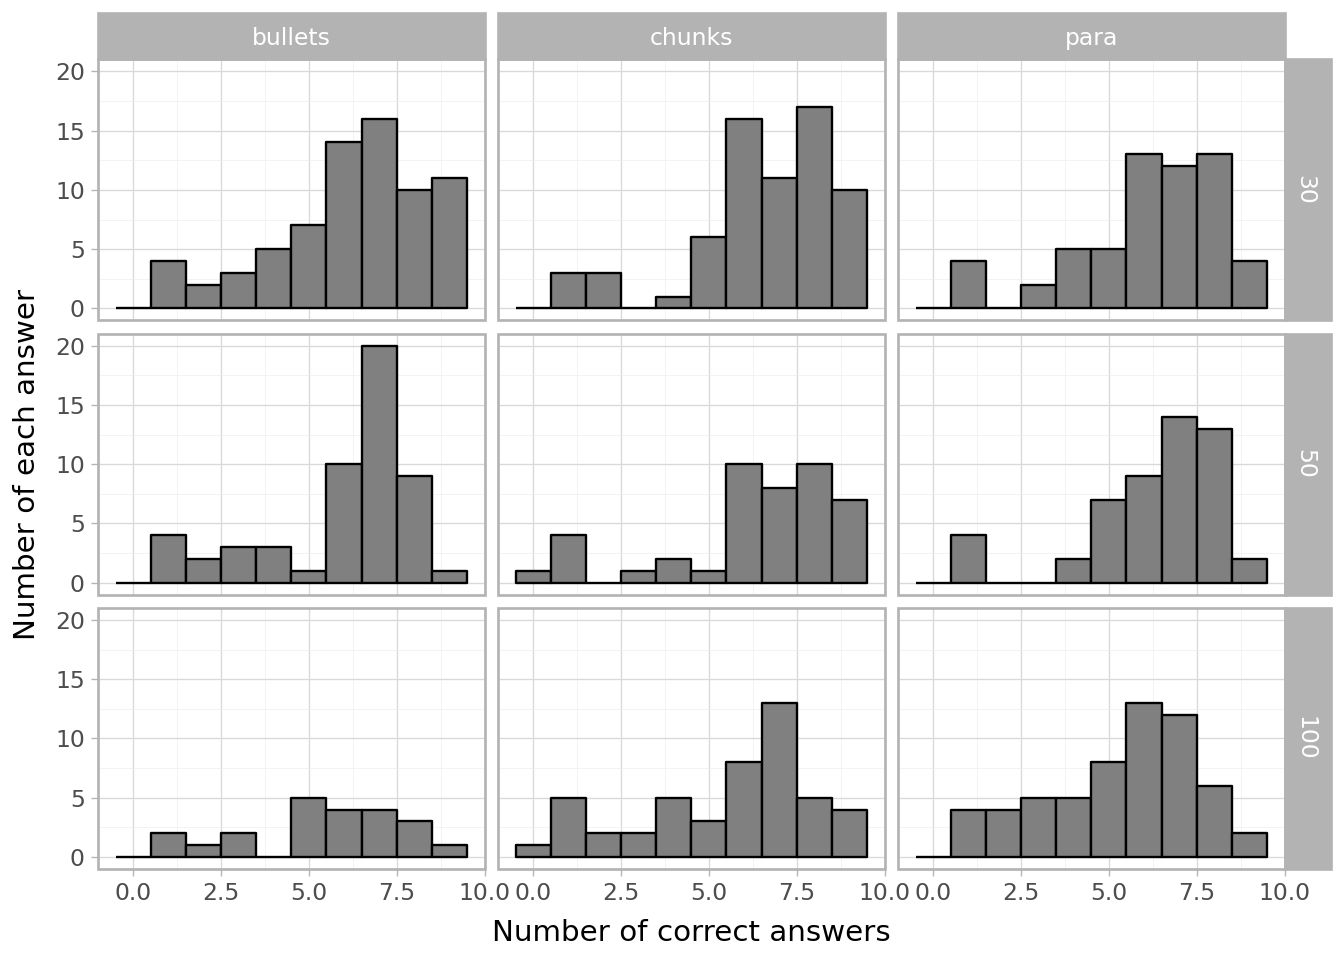
\includegraphics[width=7in,height=5in]{rieke-code_files/figure-pdf/cell-10-output-1.png}

\subsection{Total slide attractiveness
rating}\label{total-slide-attractiveness-rating}

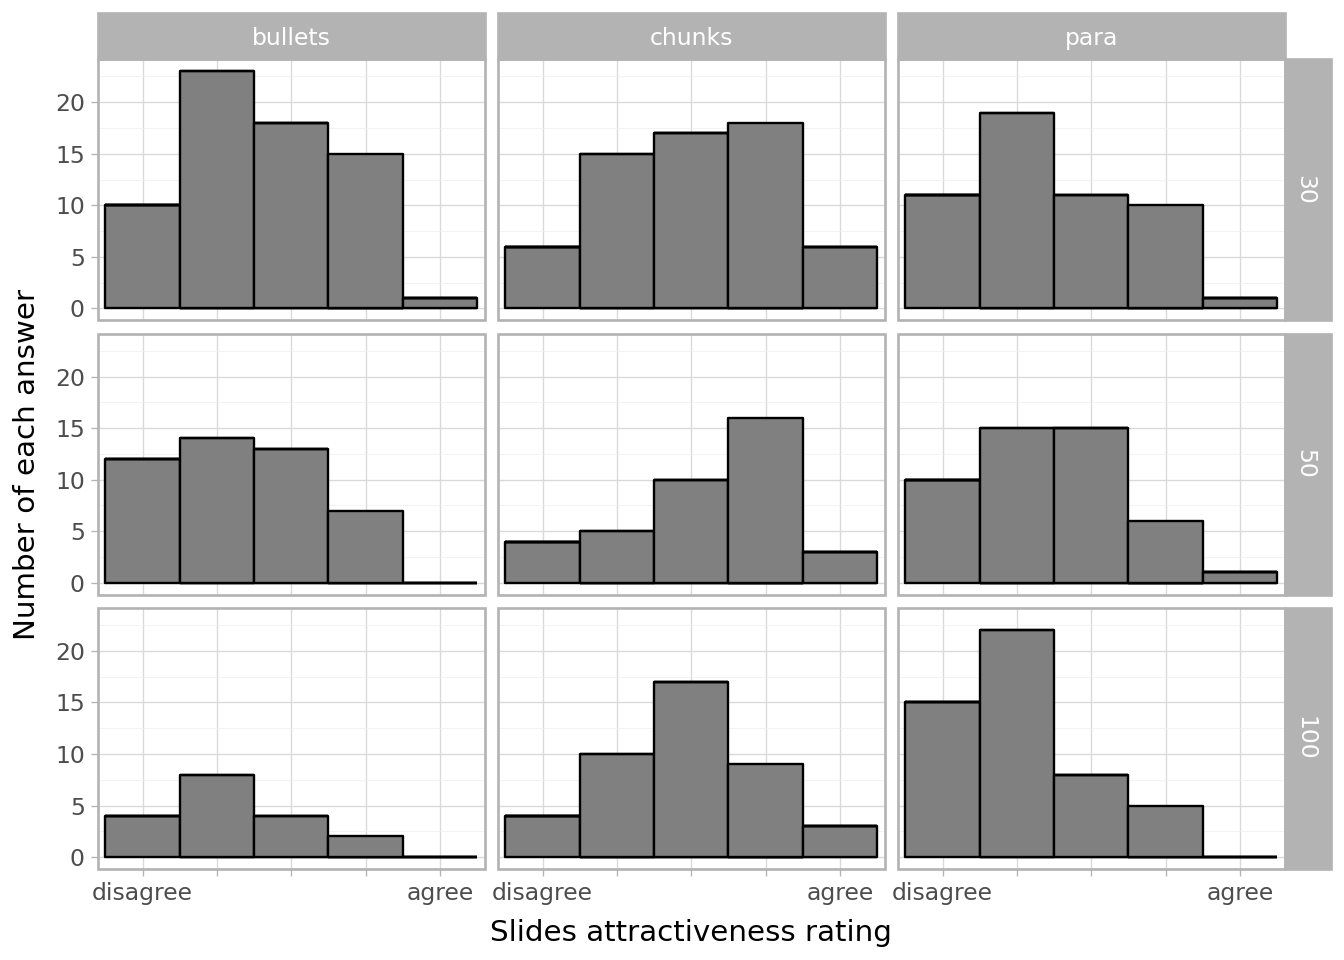
\includegraphics[width=7in,height=5in]{rieke-code_files/figure-pdf/cell-11-output-1.png}

\subsection{Total slide cleanliness
rating}\label{total-slide-cleanliness-rating}

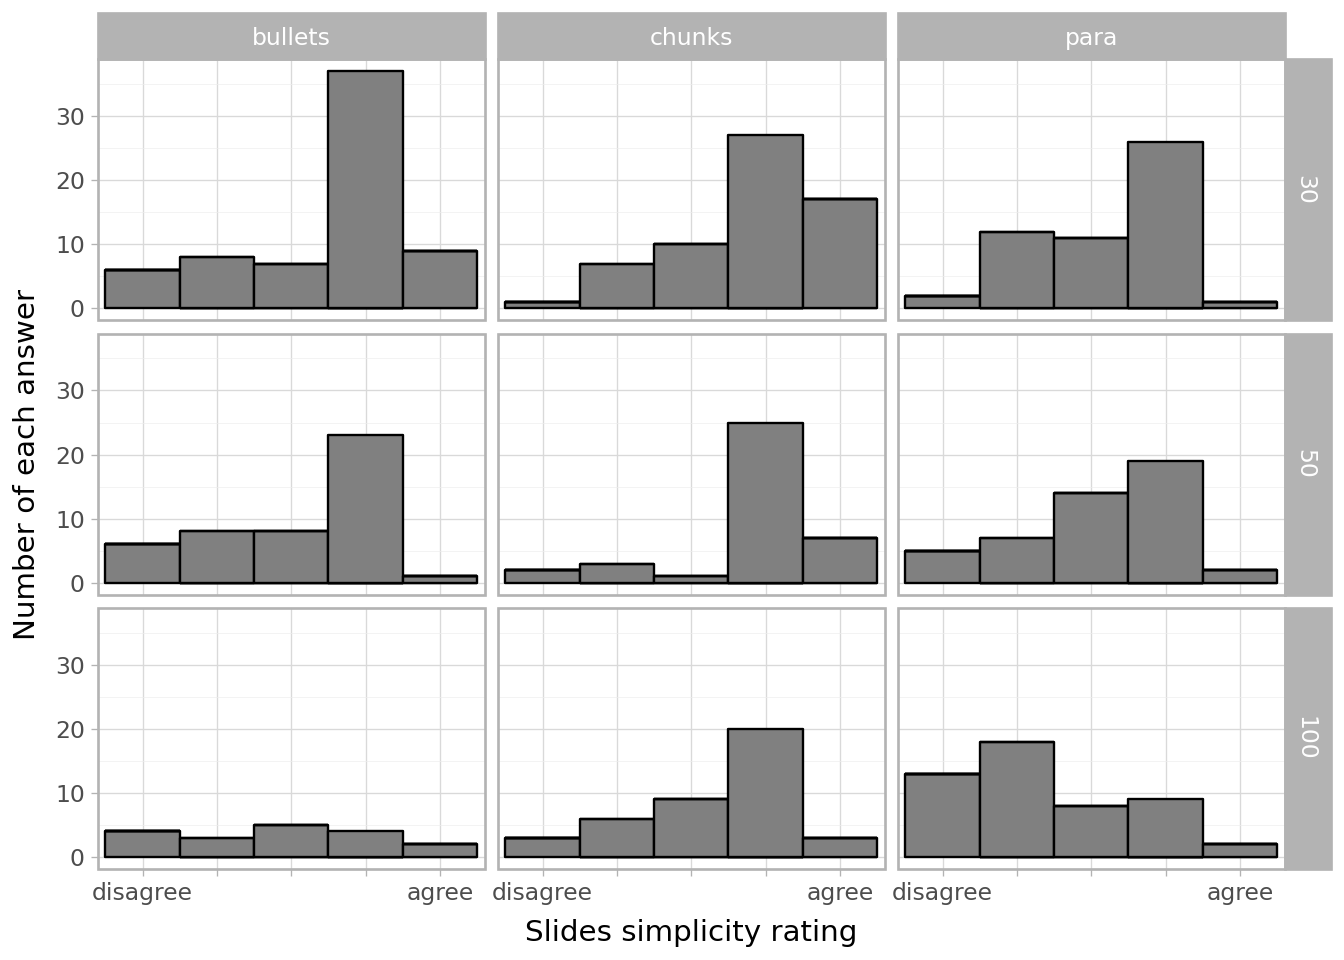
\includegraphics[width=7in,height=5in]{rieke-code_files/figure-pdf/cell-12-output-1.png}

\subsection{Total cognitive load
rating}\label{total-cognitive-load-rating}

\begin{tcolorbox}[enhanced jigsaw, arc=.35mm, bottomrule=.15mm, bottomtitle=1mm, breakable, colback=white, colbacktitle=quarto-callout-caution-color!10!white, colframe=quarto-callout-caution-color-frame, coltitle=black, left=2mm, leftrule=.75mm, opacityback=0, opacitybacktitle=0.6, rightrule=.15mm, title=\textcolor{quarto-callout-caution-color}{\faFire}\hspace{0.5em}{Caution}, titlerule=0mm, toprule=.15mm, toptitle=1mm]

Note that I swaped the x-axis to make it correspond to the previous
plots (more right = better)

\end{tcolorbox}

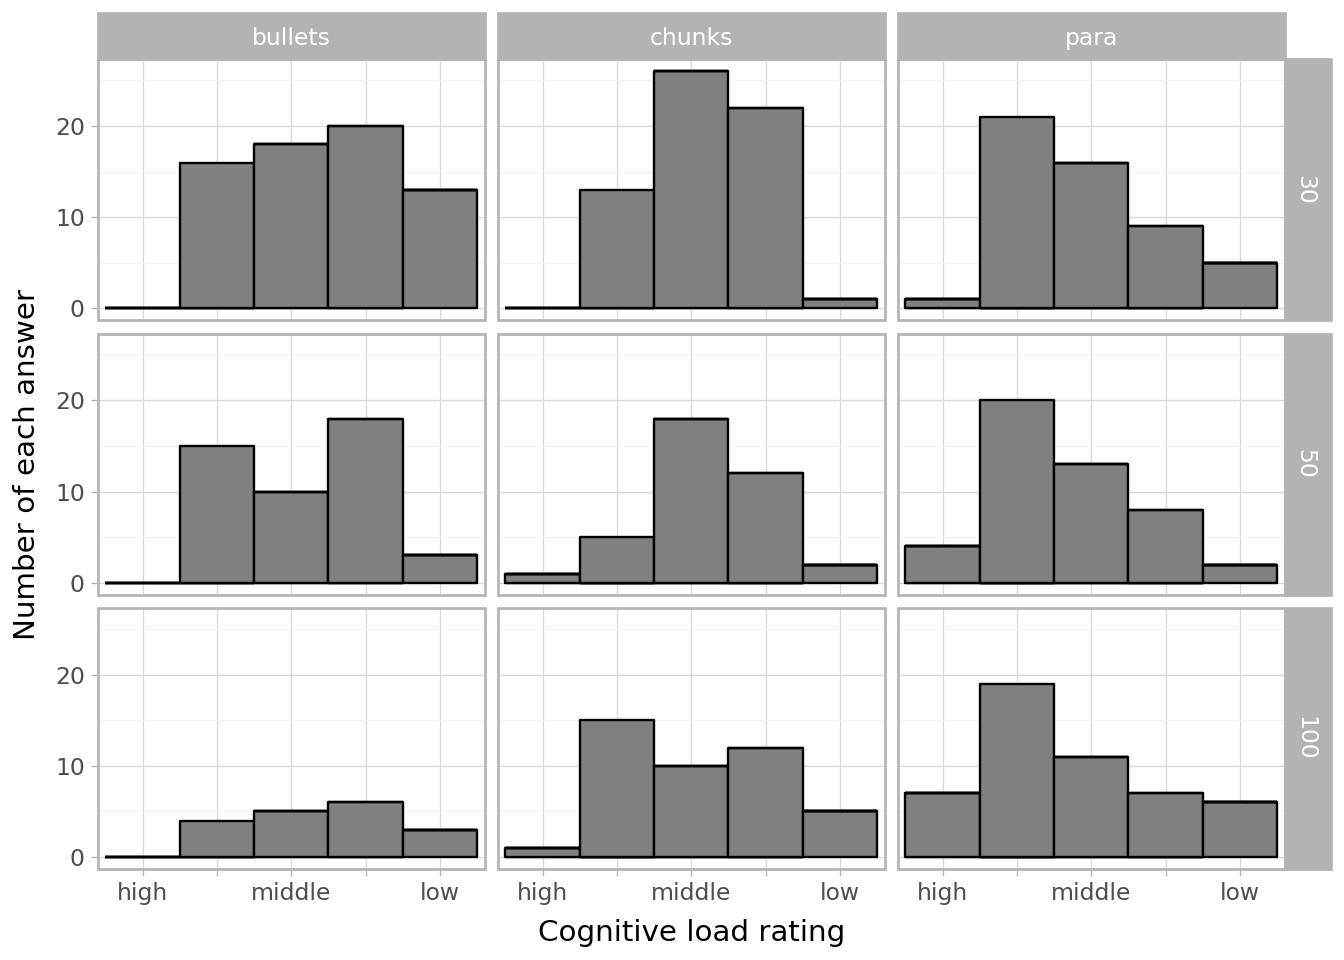
\includegraphics[width=7in,height=5in]{rieke-code_files/figure-pdf/cell-13-output-1.png}

\subsection{How many for which question
correct?}\label{how-many-for-which-question-correct}

(not corrected for missing answers!)

\begin{Shaded}
\begin{Highlighting}[]
\NormalTok{only\_correct\_counts }\OperatorTok{=}\NormalTok{ df\_combined.loc[:, df\_combined.columns.}\BuiltInTok{str}\NormalTok{.endswith(}\StringTok{\textquotesingle{}correct\textquotesingle{}}\NormalTok{) }\OperatorTok{\&} \OperatorTok{\textasciitilde{}}\NormalTok{df\_combined.columns.}\BuiltInTok{str}\NormalTok{.startswith(}\StringTok{\textquotesingle{}total\textquotesingle{}}\NormalTok{)]}
\BuiltInTok{print}\NormalTok{(only\_correct\_counts.}\BuiltInTok{sum}\NormalTok{()}\OperatorTok{/}\BuiltInTok{len}\NormalTok{(only\_correct\_counts))}
\end{Highlighting}
\end{Shaded}

\begin{verbatim}
tiger_extinct_year_correct                  0.645570
tiger_classified_correct                    0.700422
tiger_extinct_why_correct                   0.704641
why_exoplanets_important_correct            0.765823
why_prioritize_earthlike_planets_correct    0.725738
exoplanets_discovered_year_correct          0.755274
what_chatbots_reduce_correct                0.685654
what_role_crms_play_correct                 0.436709
relationship_24_7_efficiency_correct        0.616034
dtype: float64
\end{verbatim}

Order of questions 1. Tasmanian tiger 2. Exoplanets 3. AI chatbots

\section{Convert categorical data to
numbers}\label{convert-categorical-data-to-numbers}

For the statistical evaluation, the category based answers need to be
converted to numbers.

\begin{Shaded}
\begin{Highlighting}[]
\NormalTok{cognitive\_load\_scale }\OperatorTok{=}\NormalTok{ \{}
  \StringTok{"very high mental effort"}\NormalTok{: }\DecValTok{2}\NormalTok{,}
  \StringTok{"high mental effort"}\NormalTok{: }\DecValTok{1}\NormalTok{,  }
  \StringTok{"neither low nor high mental effort"}\NormalTok{: }\DecValTok{0}\NormalTok{, }
  \StringTok{"low mental effort"}\NormalTok{: }\OperatorTok{{-}}\DecValTok{1}\NormalTok{, }
  \StringTok{"very low mental effort"}\NormalTok{: }\OperatorTok{{-}}\DecValTok{2}\NormalTok{\}}

\NormalTok{slides\_scale }\OperatorTok{=}\NormalTok{ \{}\StringTok{"Strongly disagree"}\NormalTok{: }\OperatorTok{{-}}\DecValTok{2}\NormalTok{, }\StringTok{"Disagree"}\NormalTok{: }\OperatorTok{{-}}\DecValTok{1}\NormalTok{, }
  \StringTok{"Neither agree nor disagree"}\NormalTok{: }\DecValTok{0}\NormalTok{, }\StringTok{"Agree"}\NormalTok{: }\DecValTok{1}\NormalTok{, }\StringTok{"Strongly agree"}\NormalTok{: }\DecValTok{2}\NormalTok{\}}
  
\NormalTok{df\_combined[}\StringTok{\textquotesingle{}cognitive\_load\_cat\textquotesingle{}}\NormalTok{] }\OperatorTok{=}\NormalTok{ df\_combined[}\StringTok{\textquotesingle{}cognitive\_load\textquotesingle{}}\NormalTok{].}\BuiltInTok{map}\NormalTok{(cognitive\_load\_scale)}

\NormalTok{df\_combined[}\StringTok{\textquotesingle{}slides\_attractive\_cat\textquotesingle{}}\NormalTok{] }\OperatorTok{=}\NormalTok{ df\_combined[}\StringTok{\textquotesingle{}slides\_attractive\textquotesingle{}}\NormalTok{].}\BuiltInTok{map}\NormalTok{(slides\_scale)}
\NormalTok{df\_combined[}\StringTok{\textquotesingle{}slides\_clean\_simple\_cat\textquotesingle{}}\NormalTok{] }\OperatorTok{=}\NormalTok{ df\_combined[}\StringTok{\textquotesingle{}slides\_clean\_simple\textquotesingle{}}\NormalTok{].}\BuiltInTok{map}\NormalTok{(slides\_scale)}
\end{Highlighting}
\end{Shaded}

\section{Statistics}\label{statistics}

\begin{Shaded}
\begin{Highlighting}[]
\NormalTok{test\_columns }\OperatorTok{=}\NormalTok{ [}\StringTok{\textquotesingle{}total\_correct\textquotesingle{}}\NormalTok{, }
  \StringTok{\textquotesingle{}cognitive\_load\_cat\textquotesingle{}}\NormalTok{, }
  \StringTok{\textquotesingle{}slides\_attractive\_cat\textquotesingle{}}\NormalTok{, }
  \StringTok{\textquotesingle{}slides\_clean\_simple\_cat\textquotesingle{}}\NormalTok{]}
\NormalTok{test\_column\_names }\OperatorTok{=}\NormalTok{ [}\StringTok{\textquotesingle{}Correct answers\textquotesingle{}}\NormalTok{, }
  \StringTok{\textquotesingle{}Cognitive Load\textquotesingle{}}\NormalTok{, }
  \StringTok{\textquotesingle{}Slide Attractiveness\textquotesingle{}}\NormalTok{, }
  \StringTok{\textquotesingle{}Slide Simplicity\textquotesingle{}}\NormalTok{]}
\end{Highlighting}
\end{Shaded}

\subsection{sample sizes}\label{sample-sizes}

Number of answers for each question and condition combination

{\def\LTcaptype{none} % do not increment counter
\begin{longtable}[]{@{}lrrrr@{}}
\toprule\noalign{}
& Correct answers & Cognitive Load & Slide Attractiveness & Slide
Simplicity \\
\midrule\noalign{}
\endhead
\bottomrule\noalign{}
\endlastfoot
100-bullets & 22 & 18 & 18 & 18 \\
100-chunks & 48 & 43 & 43 & 41 \\
100-para & 59 & 50 & 50 & 50 \\
30-bullets & 72 & 67 & 67 & 67 \\
30-chunks & 67 & 62 & 62 & 62 \\
30-para & 58 & 52 & 52 & 52 \\
50-bullets & 53 & 46 & 46 & 46 \\
50-chunks & 44 & 38 & 38 & 38 \\
50-para & 51 & 47 & 47 & 47 \\
\end{longtable}
}

\subsection{normal distribution}\label{normal-distribution}

This is necessary to decide which test is adequate to test for a
difference between means.

\begin{tcolorbox}[enhanced jigsaw, arc=.35mm, bottomrule=.15mm, bottomtitle=1mm, breakable, colback=white, colbacktitle=quarto-callout-note-color!10!white, colframe=quarto-callout-note-color-frame, coltitle=black, left=2mm, leftrule=.75mm, opacityback=0, opacitybacktitle=0.6, rightrule=.15mm, title=\textcolor{quarto-callout-note-color}{\faInfo}\hspace{0.5em}{Note}, titlerule=0mm, toprule=.15mm, toptitle=1mm]

now Shapiro-Wilk-test (for sample size \textless50), with larger sample
size (\textgreater40) use chi-squared test or maybe also
Kolmogorov--Smirnov-test

\end{tcolorbox}

\begin{tcolorbox}[enhanced jigsaw, arc=.35mm, bottomrule=.15mm, bottomtitle=1mm, breakable, colback=white, colbacktitle=quarto-callout-tip-color!10!white, colframe=quarto-callout-tip-color-frame, coltitle=black, left=2mm, leftrule=.75mm, opacityback=0, opacitybacktitle=0.6, rightrule=.15mm, title=\textcolor{quarto-callout-tip-color}{\faLightbulb}\hspace{0.5em}{Tip}, titlerule=0mm, toprule=.15mm, toptitle=1mm]

non significant means normally distributed (or rather can't reject the
null hypothesis)

\end{tcolorbox}

\begin{Shaded}
\begin{Highlighting}[]
\NormalTok{results }\OperatorTok{=}\NormalTok{ \{\}}

\ControlFlowTok{for}\NormalTok{ column }\KeywordTok{in}\NormalTok{ test\_columns:}
\NormalTok{  new\_dict }\OperatorTok{=}\NormalTok{ \{\}}
  \ControlFlowTok{for}\NormalTok{ condition }\KeywordTok{in}\NormalTok{ condition\_list:}
\NormalTok{    df\_combined\_dropna }\OperatorTok{=}\NormalTok{ df\_combined.dropna(subset }\OperatorTok{=}\NormalTok{ [column], inplace }\OperatorTok{=} \VariableTok{False}\NormalTok{)}
\NormalTok{    S\_result, p\_value }\OperatorTok{=}\NormalTok{ stats.shapiro(df\_combined\_dropna[column][df\_combined\_dropna[}\StringTok{\textquotesingle{}condition\textquotesingle{}}\NormalTok{] }\OperatorTok{==}\NormalTok{ condition])}
\NormalTok{    new\_dict[condition] }\OperatorTok{=}\NormalTok{ \{}\StringTok{\textquotesingle{}S\_result\textquotesingle{}}\NormalTok{: S\_result, }\StringTok{\textquotesingle{}p\_value\textquotesingle{}}\NormalTok{: p\_value\}}
\NormalTok{  results[column] }\OperatorTok{=}\NormalTok{ new\_dict}
\end{Highlighting}
\end{Shaded}

\subsubsection{Correct answers}\label{correct-answers}

{\def\LTcaptype{none} % do not increment counter
\begin{longtable}[]{@{}lrr@{}}
\toprule\noalign{}
& Shapiro result statistic & p-value \\
\midrule\noalign{}
\endhead
\bottomrule\noalign{}
\endlastfoot
100-bullets & 0.928074 & 0.111871 \\
100-chunks & 0.906391 & 0.00101774 \\
100-para & 0.935612 & 0.00380742 \\
30-bullets & 0.911671 & 9.28137e-05 \\
30-chunks & 0.858825 & 1.98362e-06 \\
30-para & 0.892523 & 9.24435e-05 \\
50-bullets & 0.82047 & 1.55258e-06 \\
50-chunks & 0.839768 & 2.4236e-05 \\
50-para & 0.833444 & 4.75237e-06 \\
\end{longtable}
}

\subsubsection{Cognitive Load}\label{cognitive-load}

{\def\LTcaptype{none} % do not increment counter
\begin{longtable}[]{@{}lrr@{}}
\toprule\noalign{}
& Shapiro result statistic & p-value \\
\midrule\noalign{}
\endhead
\bottomrule\noalign{}
\endlastfoot
100-bullets & 0.885074 & 0.0318019 \\
100-chunks & 0.880614 & 0.000339894 \\
100-para & 0.886674 & 0.000179516 \\
30-bullets & 0.869574 & 4.47099e-06 \\
30-chunks & 0.836777 & 9.16678e-07 \\
30-para & 0.856992 & 1.73535e-05 \\
50-bullets & 0.833451 & 1.17254e-05 \\
50-chunks & 0.883091 & 0.000878357 \\
50-para & 0.887397 & 0.000292304 \\
\end{longtable}
}

\subsubsection{Slide Attractiveness}\label{slide-attractiveness}

{\def\LTcaptype{none} % do not increment counter
\begin{longtable}[]{@{}lrr@{}}
\toprule\noalign{}
& Shapiro result statistic & p-value \\
\midrule\noalign{}
\endhead
\bottomrule\noalign{}
\endlastfoot
100-bullets & 0.874863 & 0.0214176 \\
100-chunks & 0.916034 & 0.00398035 \\
100-para & 0.839971 & 8.37024e-06 \\
30-bullets & 0.894702 & 3.48841e-05 \\
30-chunks & 0.914255 & 0.000361399 \\
30-para & 0.88698 & 0.000137857 \\
50-bullets & 0.871061 & 0.000113873 \\
50-chunks & 0.875408 & 0.000552997 \\
50-para & 0.898979 & 0.000668267 \\
\end{longtable}
}

\subsubsection{Slide Simplicity}\label{slide-simplicity}

{\def\LTcaptype{none} % do not increment counter
\begin{longtable}[]{@{}lrr@{}}
\toprule\noalign{}
& Shapiro result statistic & p-value \\
\midrule\noalign{}
\endhead
\bottomrule\noalign{}
\endlastfoot
100-bullets & 0.910576 & 0.0880704 \\
100-chunks & 0.853085 & 8.92888e-05 \\
100-para & 0.874389 & 7.59361e-05 \\
30-bullets & 0.804395 & 5.17545e-08 \\
30-chunks & 0.855007 & 3.16259e-06 \\
30-para & 0.816589 & 1.49115e-06 \\
50-bullets & 0.809299 & 3.14212e-06 \\
50-chunks & 0.708023 & 2.2238e-07 \\
50-para & 0.869979 & 9.04645e-05 \\
\end{longtable}
}

Result: most are not normally distributed (null hypothesis rejected
within alpha 0.05)

\subsection{Mann-Whitney U-test}\label{mann-whitney-u-test}

they are not normally distributed, hence we use the U-test to test for
difference between means (variances and size of sample do not matter)

\begin{tcolorbox}[enhanced jigsaw, arc=.35mm, bottomrule=.15mm, bottomtitle=1mm, breakable, colback=white, colbacktitle=quarto-callout-tip-color!10!white, colframe=quarto-callout-tip-color-frame, coltitle=black, left=2mm, leftrule=.75mm, opacityback=0, opacitybacktitle=0.6, rightrule=.15mm, title=\textcolor{quarto-callout-tip-color}{\faLightbulb}\hspace{0.5em}{Tip}, titlerule=0mm, toprule=.15mm, toptitle=1mm]

non significant means normally distributed (or rather can't reject the
null hypothesis)

\end{tcolorbox}

\begin{tcolorbox}[enhanced jigsaw, arc=.35mm, bottomrule=.15mm, bottomtitle=1mm, breakable, colback=white, colbacktitle=quarto-callout-tip-color!10!white, colframe=quarto-callout-tip-color-frame, coltitle=black, left=2mm, leftrule=.75mm, opacityback=0, opacitybacktitle=0.6, rightrule=.15mm, title=\textcolor{quarto-callout-tip-color}{\faLightbulb}\hspace{0.5em}{Tip}, titlerule=0mm, toprule=.15mm, toptitle=1mm]

You want to look for the cases, where the p value is below 0.05. This
means there is a significant difference between the two conditions.

\end{tcolorbox}

\subsubsection{Hypothesis 1: Chunks are most
attractive}\label{hypothesis-1-chunks-are-most-attractive}

\begin{tcolorbox}[enhanced jigsaw, arc=.35mm, bottomrule=.15mm, bottomtitle=1mm, breakable, colback=white, colbacktitle=quarto-callout-important-color!10!white, colframe=quarto-callout-important-color-frame, coltitle=black, left=2mm, leftrule=.75mm, opacityback=0, opacitybacktitle=0.6, rightrule=.15mm, title=\textcolor{quarto-callout-important-color}{\faExclamation}\hspace{0.5em}{Important}, titlerule=0mm, toprule=.15mm, toptitle=1mm]

(not really a best practice to use the same dataset to develop
hypothesis and test it)

\end{tcolorbox}

\paragraph{30-chunks vs.~30-bullets}\label{chunks-vs.-30-bullets}

{\def\LTcaptype{none} % do not increment counter
\begin{longtable}[]{@{}lrr@{}}
\toprule\noalign{}
& U1\_stat & p\_value \\
\midrule\noalign{}
\endhead
\bottomrule\noalign{}
\endlastfoot
Correct answers & 2675.5 & 0.269437 \\
Cognitive Load & 2371.5 & 0.167041 \\
Slide Attractiveness & 2518.5 & 0.0375491 \\
Slide Simplicity & 2377 & 0.158495 \\
\end{longtable}
}

\paragraph{30-chunks vs.~30-para}\label{chunks-vs.-30-para}

{\def\LTcaptype{none} % do not increment counter
\begin{longtable}[]{@{}lrr@{}}
\toprule\noalign{}
& U1\_stat & p\_value \\
\midrule\noalign{}
\endhead
\bottomrule\noalign{}
\endlastfoot
Correct answers & 2220 & 0.171644 \\
Cognitive Load & 1310 & 0.0863214 \\
Slide Attractiveness & 2081 & 0.00735154 \\
Slide Simplicity & 2153.5 & 0.00191711 \\
\end{longtable}
}

\paragraph{50-chunks vs.~50-bullets}\label{chunks-vs.-50-bullets}

{\def\LTcaptype{none} % do not increment counter
\begin{longtable}[]{@{}lrr@{}}
\toprule\noalign{}
& U1\_stat & p\_value \\
\midrule\noalign{}
\endhead
\bottomrule\noalign{}
\endlastfoot
Correct answers & 1335.5 & 0.223198 \\
Cognitive Load & 853.5 & 0.861631 \\
Slide Attractiveness & 1262 & 0.00039186 \\
Slide Simplicity & 1210 & 0.00228298 \\
\end{longtable}
}

\paragraph{50-chunks vs.~50-para}\label{chunks-vs.-50-para}

{\def\LTcaptype{none} % do not increment counter
\begin{longtable}[]{@{}lrr@{}}
\toprule\noalign{}
& U1\_stat & p\_value \\
\midrule\noalign{}
\endhead
\bottomrule\noalign{}
\endlastfoot
Correct answers & 1213.5 & 0.501142 \\
Cognitive Load & 581 & 0.00548155 \\
Slide Attractiveness & 1260 & 0.0010141 \\
Slide Simplicity & 1259 & 0.00104827 \\
\end{longtable}
}

\paragraph{100-chunks vs.~100-bullets}\label{chunks-vs.-100-bullets}

{\def\LTcaptype{none} % do not increment counter
\begin{longtable}[]{@{}lrr@{}}
\toprule\noalign{}
& U1\_stat & p\_value \\
\midrule\noalign{}
\endhead
\bottomrule\noalign{}
\endlastfoot
Correct answers & 553 & 0.758391 \\
Cognitive Load & 452.5 & 0.310775 \\
Slide Attractiveness & 533 & 0.0204201 \\
Slide Simplicity & 455.5 & 0.160662 \\
\end{longtable}
}

\paragraph{100-chunks vs.~100-para}\label{chunks-vs.-100-para}

{\def\LTcaptype{none} % do not increment counter
\begin{longtable}[]{@{}lrr@{}}
\toprule\noalign{}
& U1\_stat & p\_value \\
\midrule\noalign{}
\endhead
\bottomrule\noalign{}
\endlastfoot
Correct answers & 1533.5 & 0.467138 \\
Cognitive Load & 863 & 0.103354 \\
Slide Attractiveness & 1564.5 & 0.000123269 \\
Slide Simplicity & 1483.5 & 0.000200477 \\
\end{longtable}
}

\subsubsection{Hypothesis 2: Bullets worse the
longer}\label{hypothesis-2-bullets-worse-the-longer}

\paragraph{30-bullets vs.~50-bullets}\label{bullets-vs.-50-bullets}

{\def\LTcaptype{none} % do not increment counter
\begin{longtable}[]{@{}lrr@{}}
\toprule\noalign{}
& U1\_stat & p\_value \\
\midrule\noalign{}
\endhead
\bottomrule\noalign{}
\endlastfoot
Correct answers & 2013 & 0.602865 \\
Cognitive Load & 1343.5 & 0.251936 \\
Slide Attractiveness & 1765.5 & 0.192307 \\
Slide Simplicity & 1873 & 0.0524509 \\
\end{longtable}
}

\paragraph{30-bullets vs.~100-bullets}\label{bullets-vs.-100-bullets}

{\def\LTcaptype{none} % do not increment counter
\begin{longtable}[]{@{}lrr@{}}
\toprule\noalign{}
& U1\_stat & p\_value \\
\midrule\noalign{}
\endhead
\bottomrule\noalign{}
\endlastfoot
Correct answers & 954 & 0.150185 \\
Cognitive Load & 602.5 & 1 \\
Slide Attractiveness & 729 & 0.178583 \\
Slide Simplicity & 793.5 & 0.0407951 \\
\end{longtable}
}

\paragraph{50-bullets vs.~100-bullets}\label{bullets-vs.-100-bullets-1}

{\def\LTcaptype{none} % do not increment counter
\begin{longtable}[]{@{}lrr@{}}
\toprule\noalign{}
& U1\_stat & p\_value \\
\midrule\noalign{}
\endhead
\bottomrule\noalign{}
\endlastfoot
Correct answers & 680.5 & 0.263618 \\
Cognitive Load & 467.5 & 0.436522 \\
Slide Attractiveness & 437 & 0.73917 \\
Slide Simplicity & 471 & 0.402249 \\
\end{longtable}
}

\subsubsection{Hypothesis 3: Long chunks don't
work}\label{hypothesis-3-long-chunks-dont-work}

see Hypothesis 1

\subsubsection{other stuff}\label{other-stuff}

comparing the most extreme conditions

\paragraph{30-chunks vs.~100-bullets}\label{chunks-vs.-100-bullets-1}

{\def\LTcaptype{none} % do not increment counter
\begin{longtable}[]{@{}lrr@{}}
\toprule\noalign{}
& U1\_stat & p\_value \\
\midrule\noalign{}
\endhead
\bottomrule\noalign{}
\endlastfoot
Correct answers & 975 & 0.023139 \\
Cognitive Load & 640.5 & 0.350803 \\
Slide Attractiveness & 784 & 0.00855091 \\
Slide Simplicity & 802.5 & 0.00436971 \\
\end{longtable}
}

\paragraph{30-bullets vs.~100-bullets}\label{bullets-vs.-100-bullets-2}

{\def\LTcaptype{none} % do not increment counter
\begin{longtable}[]{@{}lrr@{}}
\toprule\noalign{}
& U1\_stat & p\_value \\
\midrule\noalign{}
\endhead
\bottomrule\noalign{}
\endlastfoot
Correct answers & 954 & 0.150185 \\
Cognitive Load & 602.5 & 1 \\
Slide Attractiveness & 729 & 0.178583 \\
Slide Simplicity & 793.5 & 0.0407951 \\
\end{longtable}
}

\subsection{Explorations}\label{explorations}

\begin{tcolorbox}[enhanced jigsaw, arc=.35mm, bottomrule=.15mm, bottomtitle=1mm, breakable, colback=white, colbacktitle=quarto-callout-tip-color!10!white, colframe=quarto-callout-tip-color-frame, coltitle=black, left=2mm, leftrule=.75mm, opacityback=0, opacitybacktitle=0.6, rightrule=.15mm, title=\textcolor{quarto-callout-tip-color}{\faLightbulb}\hspace{0.5em}{Tip}, titlerule=0mm, toprule=.15mm, toptitle=1mm]

There are violin plots with an overlay box plot in this section. See for
example
\href{https://mode.com/blog/violin-plot-examples\#how-to-read-violin-plot}{here}
for an explanation how to read it. In the other plots (beeswarm plots)
each point corresponds to one answer. They are slightly offset in
x-direction to make it easier to see.

\end{tcolorbox}

\subsubsection{Correlation between cognitive load and correct
answers?}\label{correlation-between-cognitive-load-and-correct-answers}

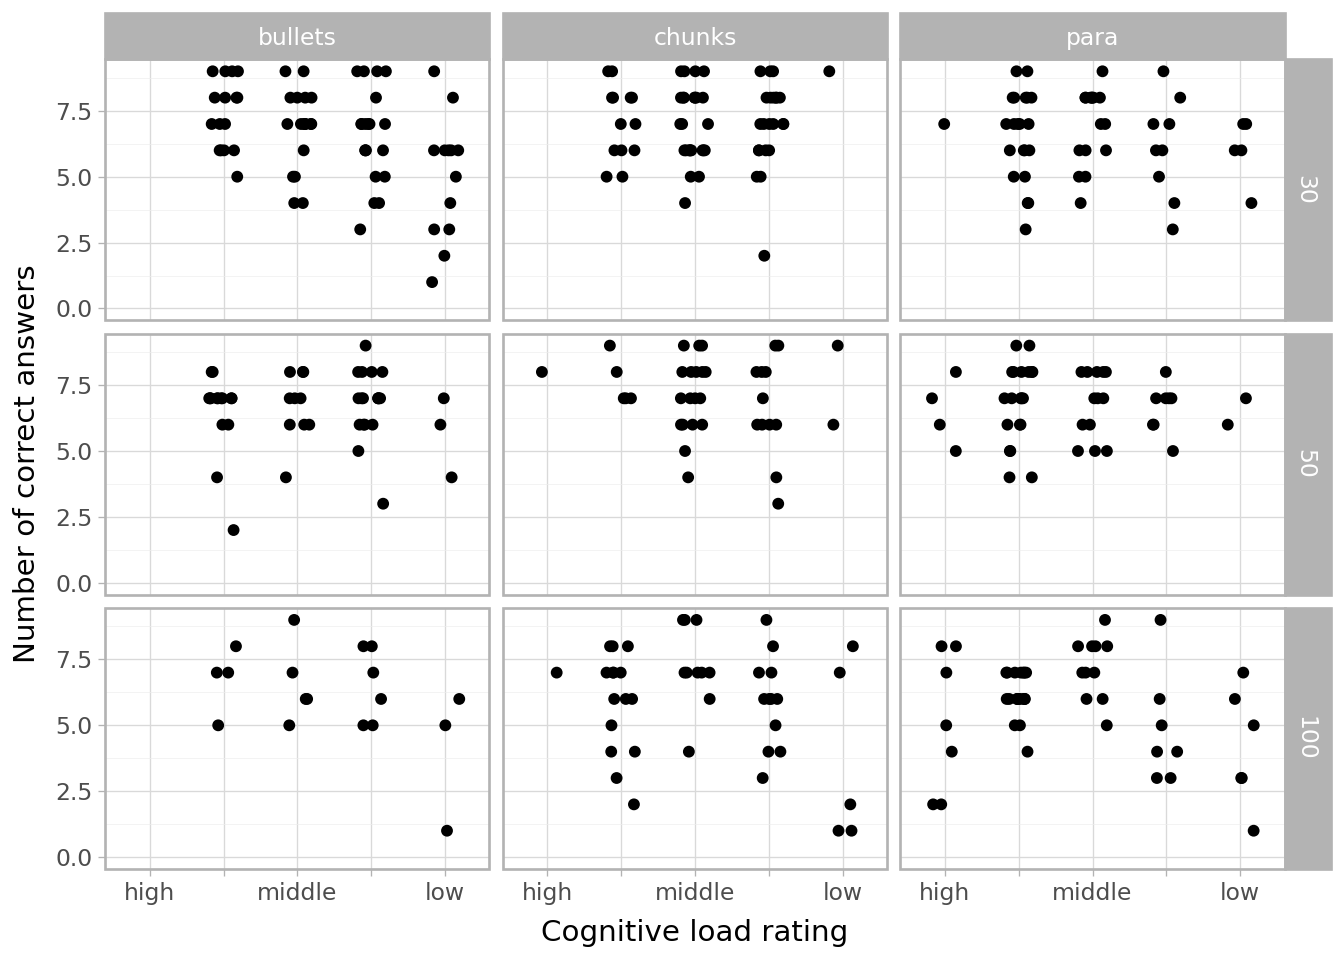
\includegraphics[width=7in,height=5in]{rieke-code_files/figure-pdf/cell-31-output-1.png}

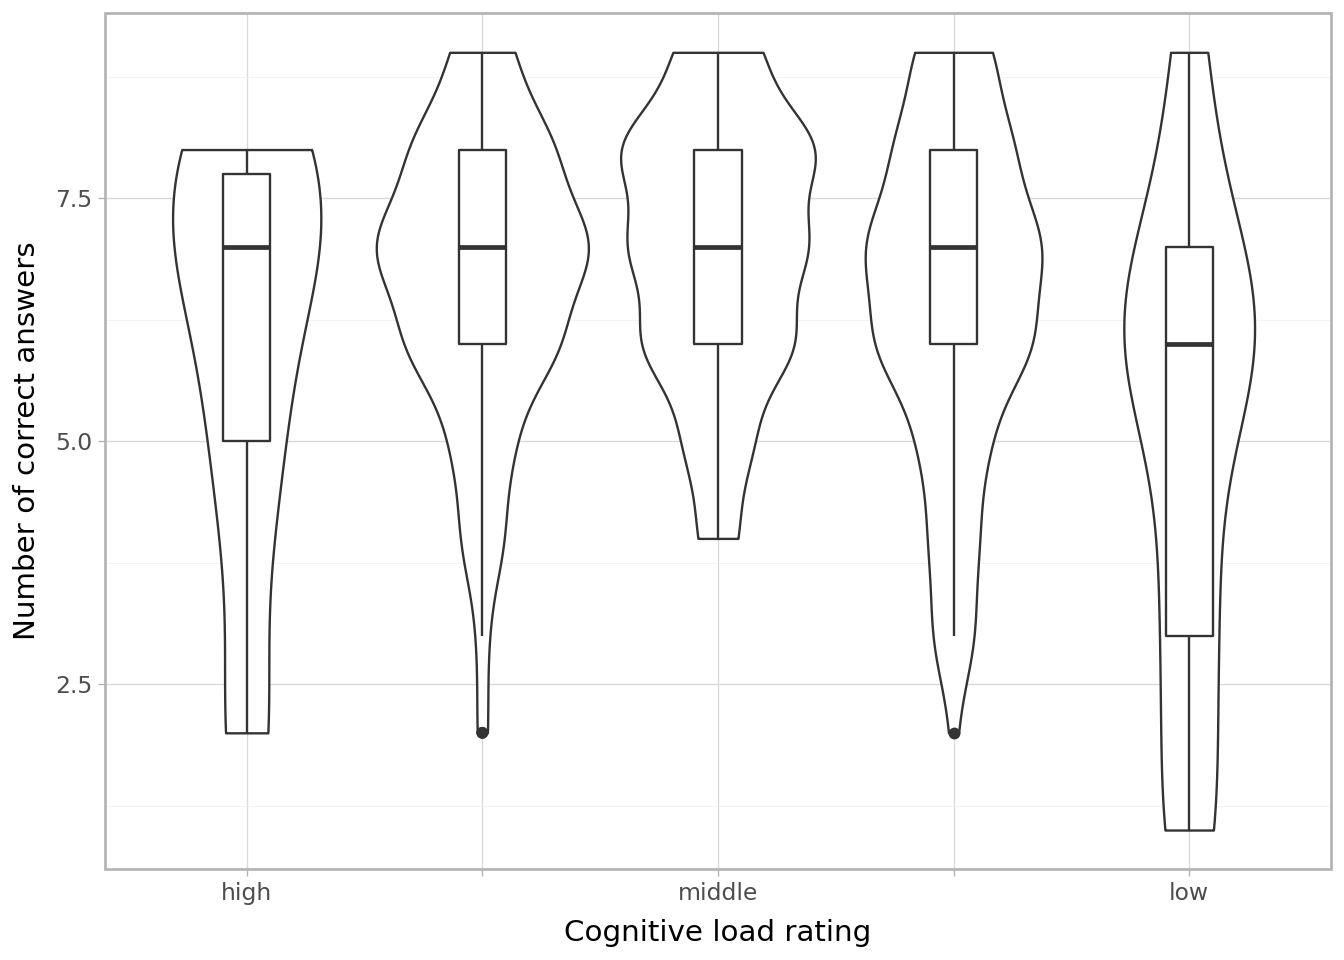
\includegraphics[width=7in,height=5in]{rieke-code_files/figure-pdf/cell-32-output-1.png}

\subsubsection{Correlation between slide simplicity and correct
answers?}\label{correlation-between-slide-simplicity-and-correct-answers}

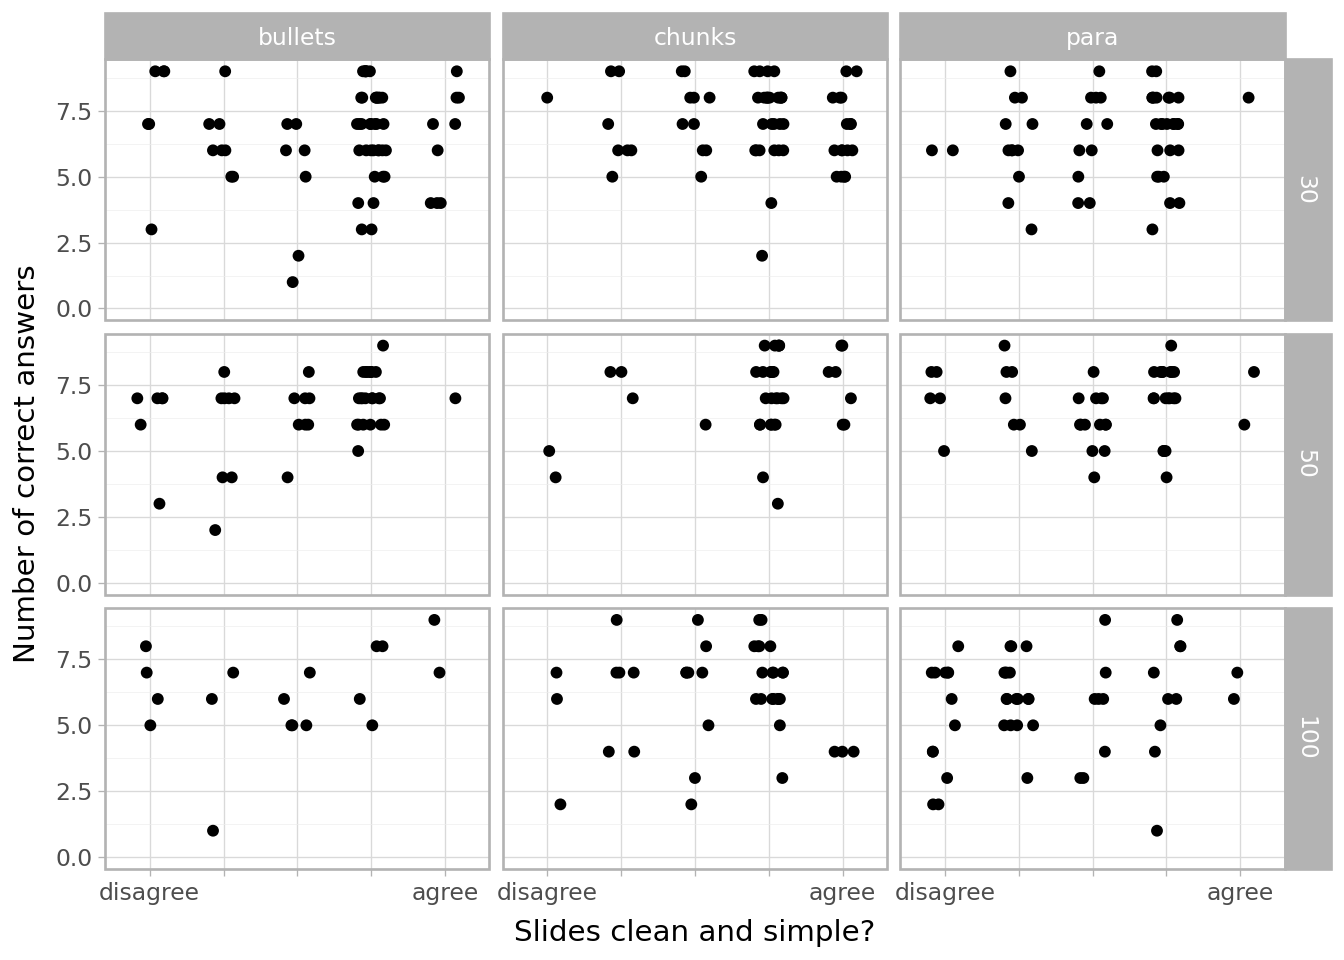
\includegraphics[width=7in,height=5in]{rieke-code_files/figure-pdf/cell-33-output-1.png}

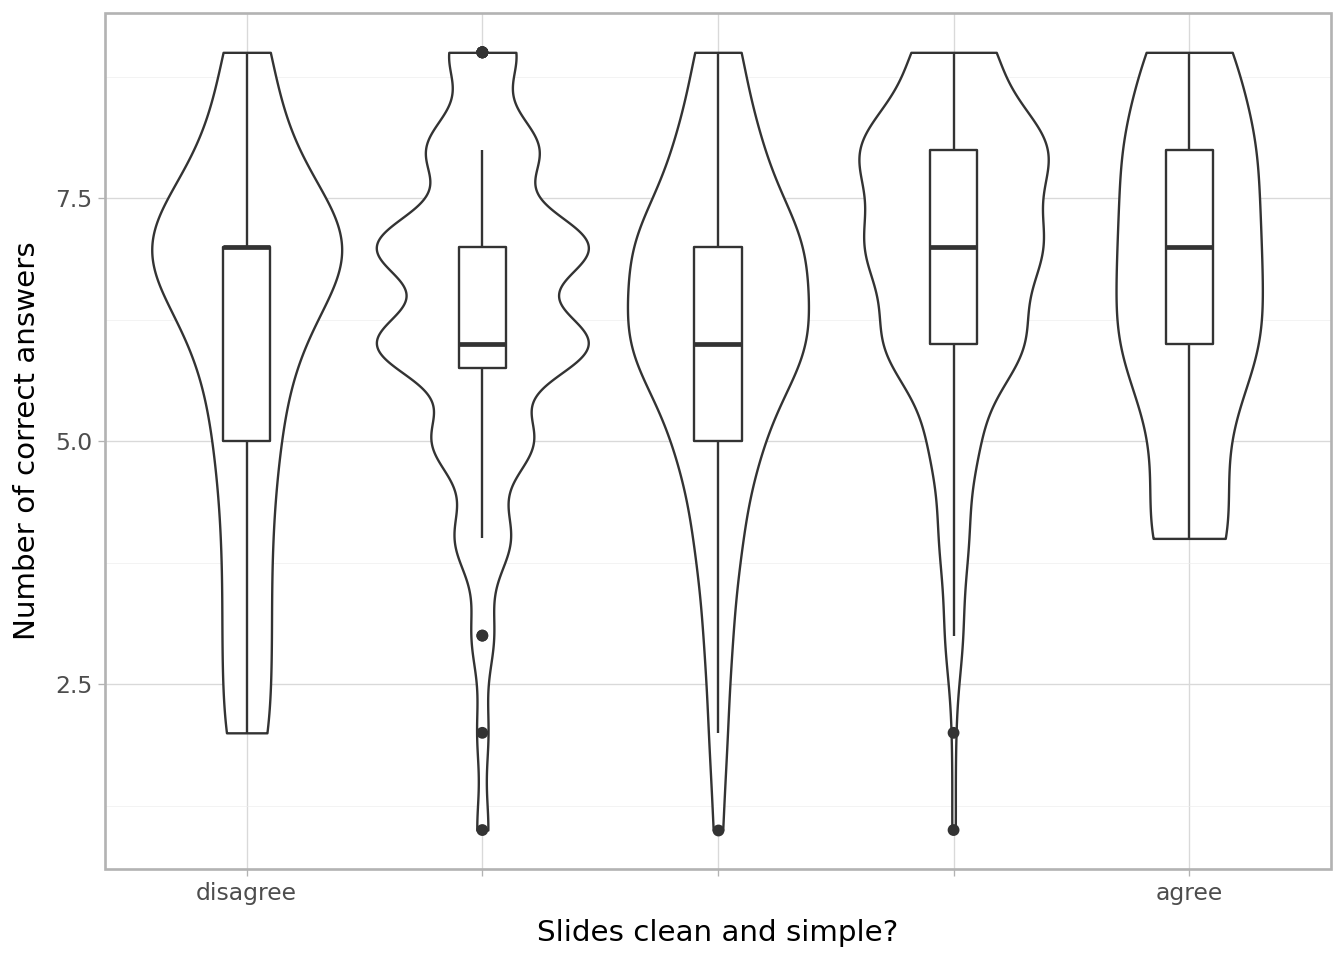
\includegraphics[width=7in,height=5in]{rieke-code_files/figure-pdf/cell-34-output-1.png}

\subsubsection{Correlation between slide attractiveness and correct
answers?}\label{correlation-between-slide-attractiveness-and-correct-answers}

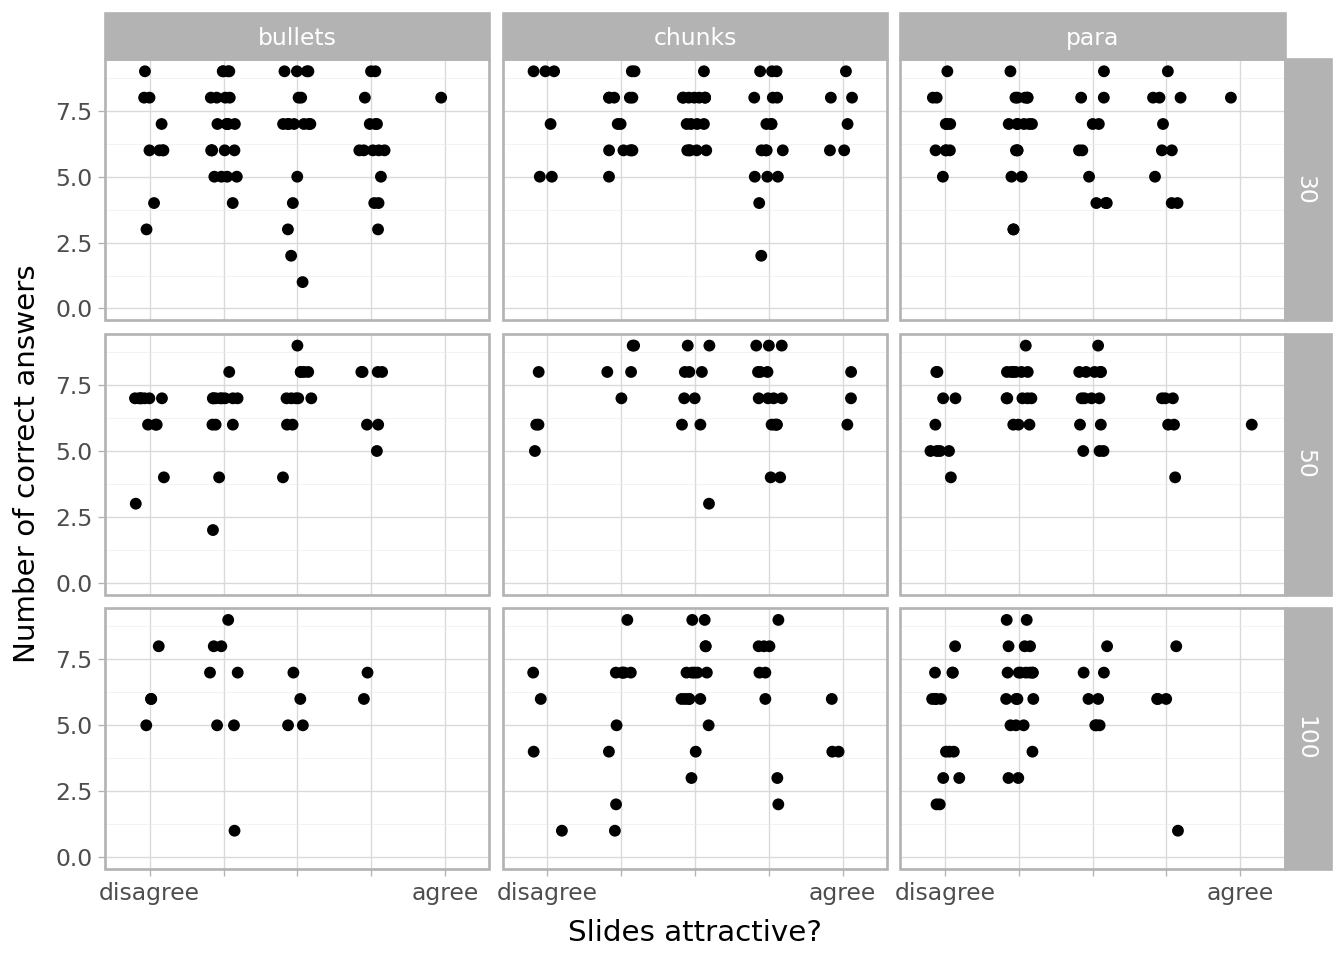
\includegraphics[width=7in,height=5in]{rieke-code_files/figure-pdf/cell-35-output-1.png}

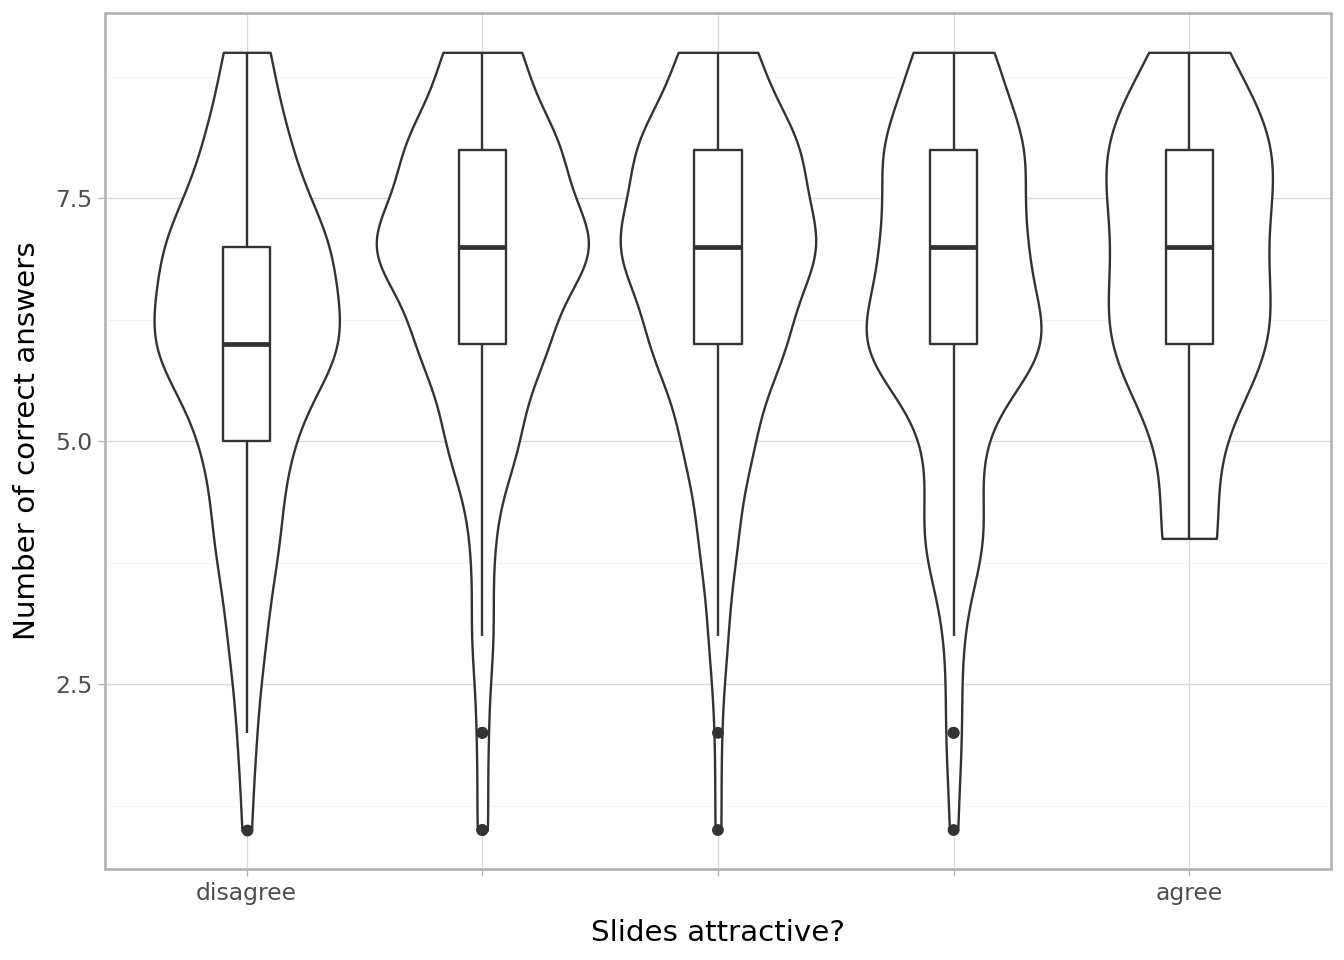
\includegraphics[width=7in,height=5in]{rieke-code_files/figure-pdf/cell-36-output-1.png}

\subsubsection{Who stopped answering
when?}\label{who-stopped-answering-when}

Number of people starting in each condition

\begin{verbatim}
condition
100-bullets    22
100-chunks     48
100-para       59
30-bullets     72
30-chunks      67
30-para        58
50-bullets     53
50-chunks      44
50-para        51
dtype: Int64
\end{verbatim}

Number of people who answered each question per condition

{\def\LTcaptype{none} % do not increment counter
\begin{longtable}[]{@{}llll@{}}
\toprule\noalign{}
& tiger\_extinct\_year & why\_exoplanets\_important &
what\_chatbots\_reduce \\
condition & & & \\
\midrule\noalign{}
\endhead
\bottomrule\noalign{}
\endlastfoot
100-bullets & 22 & 22 & 22 \\
100-chunks & 48 & 48 & 48 \\
100-para & 59 & 59 & 59 \\
30-bullets & 72 & 72 & 72 \\
30-chunks & 67 & 67 & 67 \\
30-para & 58 & 58 & 58 \\
50-bullets & 53 & 53 & 53 \\
50-chunks & 44 & 44 & 44 \\
50-para & 51 & 51 & 51 \\
\end{longtable}
}

As the answer numbers per question theme is the same, I chose just one
question in each theme to count the answers.

There doesn't seem to emerge a clear pattern (except maybe for the
paragraphs where in each condition the same number of people dropped out
after each question, but with that sample size that might just be
chance).

\subsubsection{Number of correct answers to first
questions?}\label{number-of-correct-answers-to-first-questions}

This is the number of correct answers for the first theme (total number,
not relative amount to the people that actually answered -- check the
table above for an idea how many people answered).

{\def\LTcaptype{none} % do not increment counter
\begin{longtable}[]{@{}llll@{}}
\toprule\noalign{}
& tiger\_classified\_correct & tiger\_extinct\_year\_correct &
tiger\_extinct\_why\_correct \\
condition & & & \\
\midrule\noalign{}
\endhead
\bottomrule\noalign{}
\endlastfoot
100-bullets & 20 & 15 & 15 \\
100-chunks & 37 & 26 & 22 \\
100-para & 46 & 31 & 40 \\
30-bullets & 44 & 52 & 51 \\
30-chunks & 51 & 49 & 53 \\
30-para & 37 & 31 & 42 \\
50-bullets & 33 & 36 & 40 \\
50-chunks & 27 & 32 & 34 \\
50-para & 37 & 34 & 37 \\
\end{longtable}
}

In contrast, the number of correct answers for the following themes:

{\def\LTcaptype{none} % do not increment counter
\begin{longtable}[]{@{}llll@{}}
\toprule\noalign{}
& why\_exoplanets\_important\_correct &
why\_prioritize\_earthlike\_planets\_correct &
exoplanets\_discovered\_year\_correct \\
condition & & & \\
\midrule\noalign{}
\endhead
\bottomrule\noalign{}
\endlastfoot
100-bullets & 17 & 14 & 14 \\
100-chunks & 37 & 31 & 29 \\
100-para & 45 & 41 & 36 \\
30-bullets & 52 & 53 & 58 \\
30-chunks & 49 & 54 & 57 \\
30-para & 44 & 44 & 47 \\
50-bullets & 42 & 41 & 40 \\
50-chunks & 37 & 29 & 37 \\
50-para & 40 & 37 & 40 \\
\end{longtable}
}

{\def\LTcaptype{none} % do not increment counter
\begin{longtable}[]{@{}llll@{}}
\toprule\noalign{}
& what\_chatbots\_reduce\_correct & what\_role\_crms\_play\_correct &
relationship\_24\_7\_efficiency\_correct \\
condition & & & \\
\midrule\noalign{}
\endhead
\bottomrule\noalign{}
\endlastfoot
100-bullets & 10 & 4 & 11 \\
100-chunks & 36 & 21 & 26 \\
100-para & 28 & 13 & 35 \\
30-bullets & 52 & 42 & 43 \\
30-chunks & 54 & 39 & 36 \\
30-para & 43 & 28 & 41 \\
50-bullets & 31 & 20 & 32 \\
50-chunks & 32 & 24 & 27 \\
50-para & 39 & 16 & 41 \\
\end{longtable}
}

\section{Main Effects}\label{main-effects}

The previous analysis used pairwise comparisons. Here, we test for the
main effects of slide length and format, as well as their interaction,
on our outcome variables.

This section moves from condition-by-condition comparisons to a
model-based view of the 3x3 design, so we can see whether length,
format, or their interaction explains the outcomes.

\subsubsection{Learning / correct
answers}\label{learning-correct-answers}

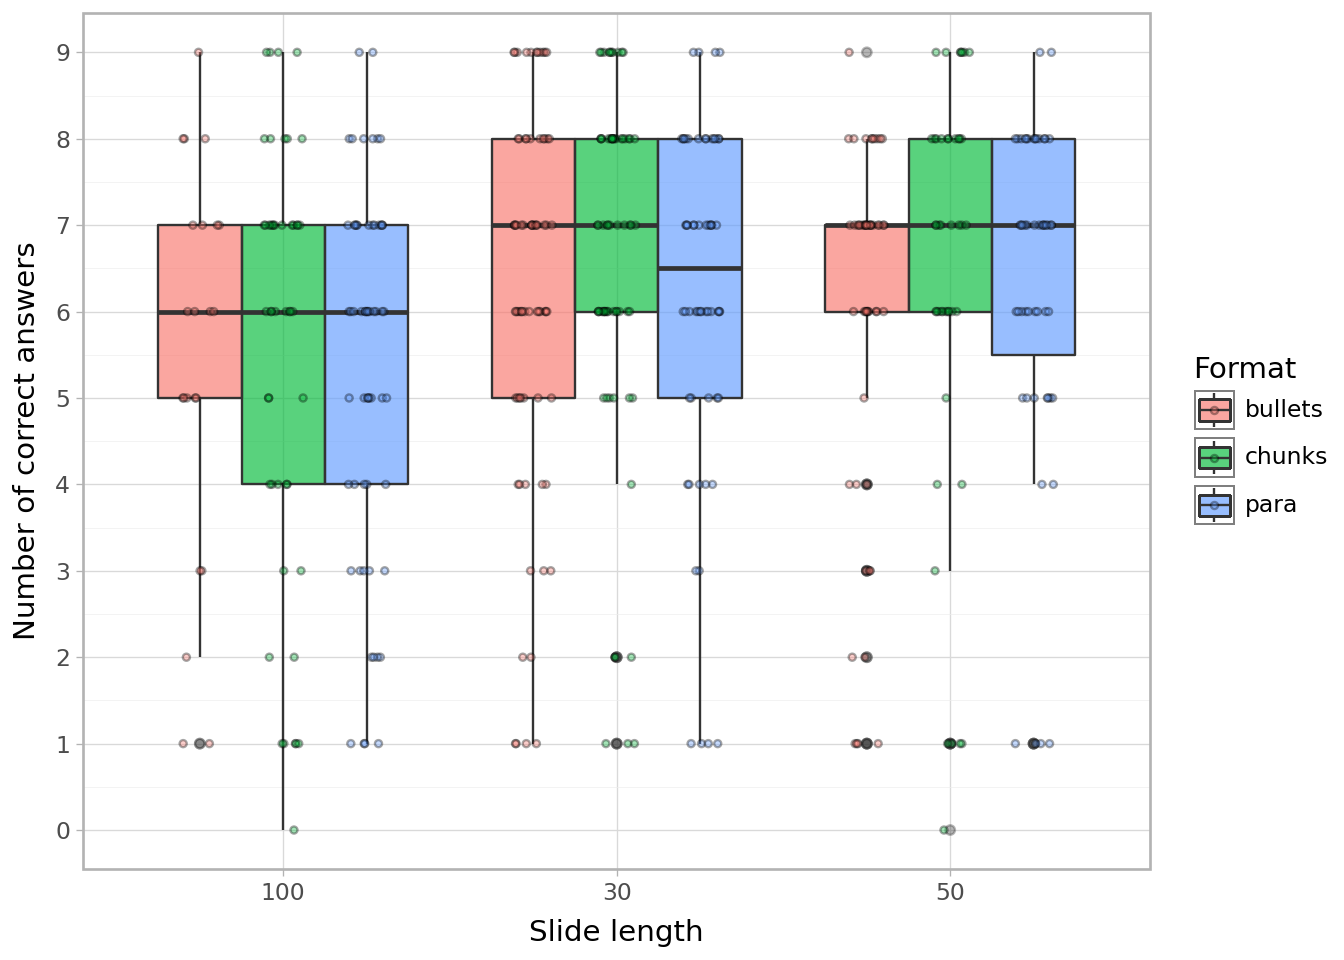
\includegraphics[width=7in,height=5in]{rieke-code_files/figure-pdf/cell-42-output-2.png}

\textbf{Main effects table}

{\def\LTcaptype{none} % do not increment counter
\begin{longtable}[]{@{}lrrl@{}}
\toprule\noalign{}
Effect & F & p\_value & Significant \\
\midrule\noalign{}
\endhead
\bottomrule\noalign{}
\endlastfoot
Slide length & 7.28872 & 0.000764105 & Yes \\
Format & 0.945931 & 0.389064 & No \\
Length x format & 0.224262 & 0.924832 & No \\
\end{longtable}
}

\textbf{Overall, longer slides hurt learning.}

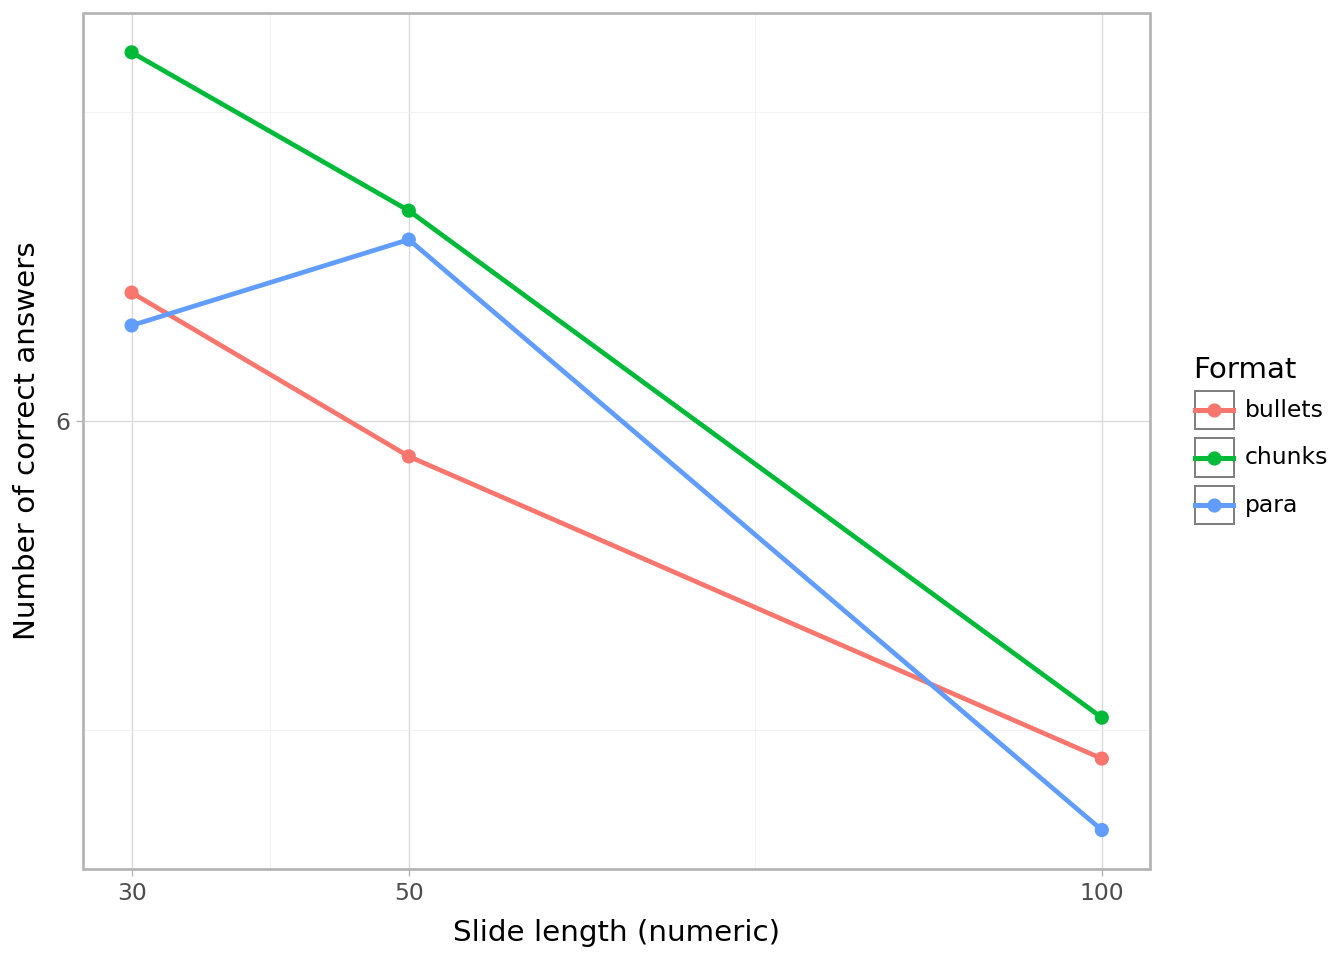
\includegraphics[width=7in,height=5in]{rieke-code_files/figure-pdf/cell-42-output-6.png}

\begin{tcolorbox}[enhanced jigsaw, arc=.35mm, bottomrule=.15mm, bottomtitle=1mm, breakable, colback=white, colbacktitle=quarto-callout-caution-color!10!white, colframe=quarto-callout-caution-color-frame, coltitle=black, left=2mm, leftrule=.75mm, opacityback=0, opacitybacktitle=0.6, rightrule=.15mm, title=\textcolor{quarto-callout-caution-color}{\faFire}\hspace{0.5em}{Caution}, titlerule=0mm, toprule=.15mm, toptitle=1mm]

This numeric trend plot treats slide length as a continuous predictor
and assumes a linear trend across 30, 50, and 100. In this study, slide
length was experimentally manipulated in discrete categories, so this
plot is best interpreted as a descriptive trend view rather than
definitive evidence of linearity.

\end{tcolorbox}

\begin{verbatim}
 
\end{verbatim}

\subsubsection{Appeal / slide
attractiveness}\label{appeal-slide-attractiveness}

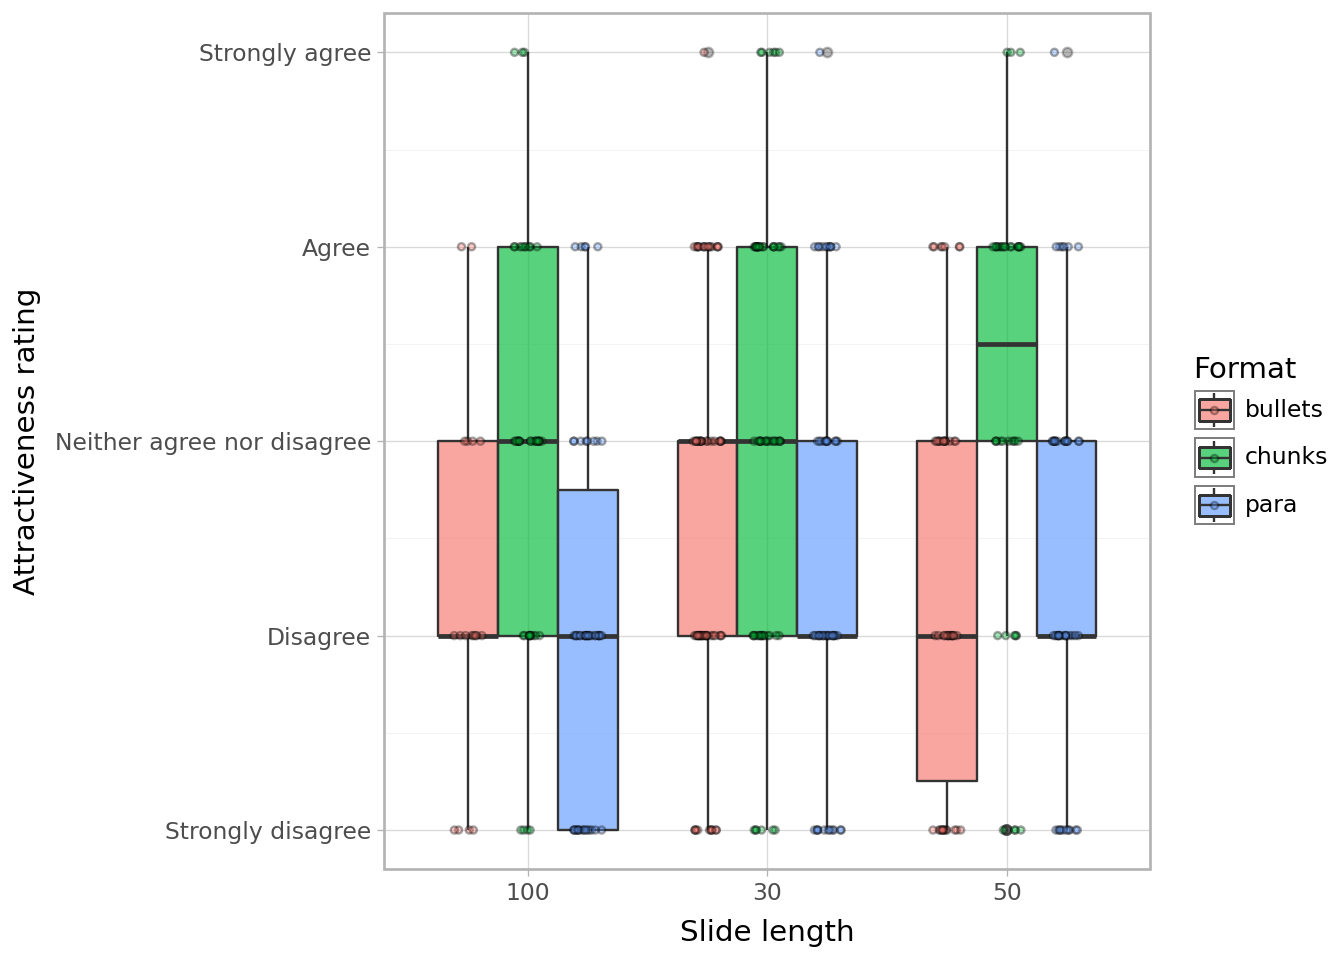
\includegraphics[width=7in,height=5in]{rieke-code_files/figure-pdf/cell-42-output-10.png}

\textbf{Main effects table}

{\def\LTcaptype{none} % do not increment counter
\begin{longtable}[]{@{}lrrl@{}}
\toprule\noalign{}
Effect & F & p\_value & Significant \\
\midrule\noalign{}
\endhead
\bottomrule\noalign{}
\endlastfoot
Slide length & 2.91619 & 0.0552526 & No \\
Format & 20.844 & 2.37078e-09 & Yes \\
Length x format & 0.771858 & 0.543968 & No \\
\end{longtable}
}

\textbf{Overall, longer slides reduce perceived attractiveness.}

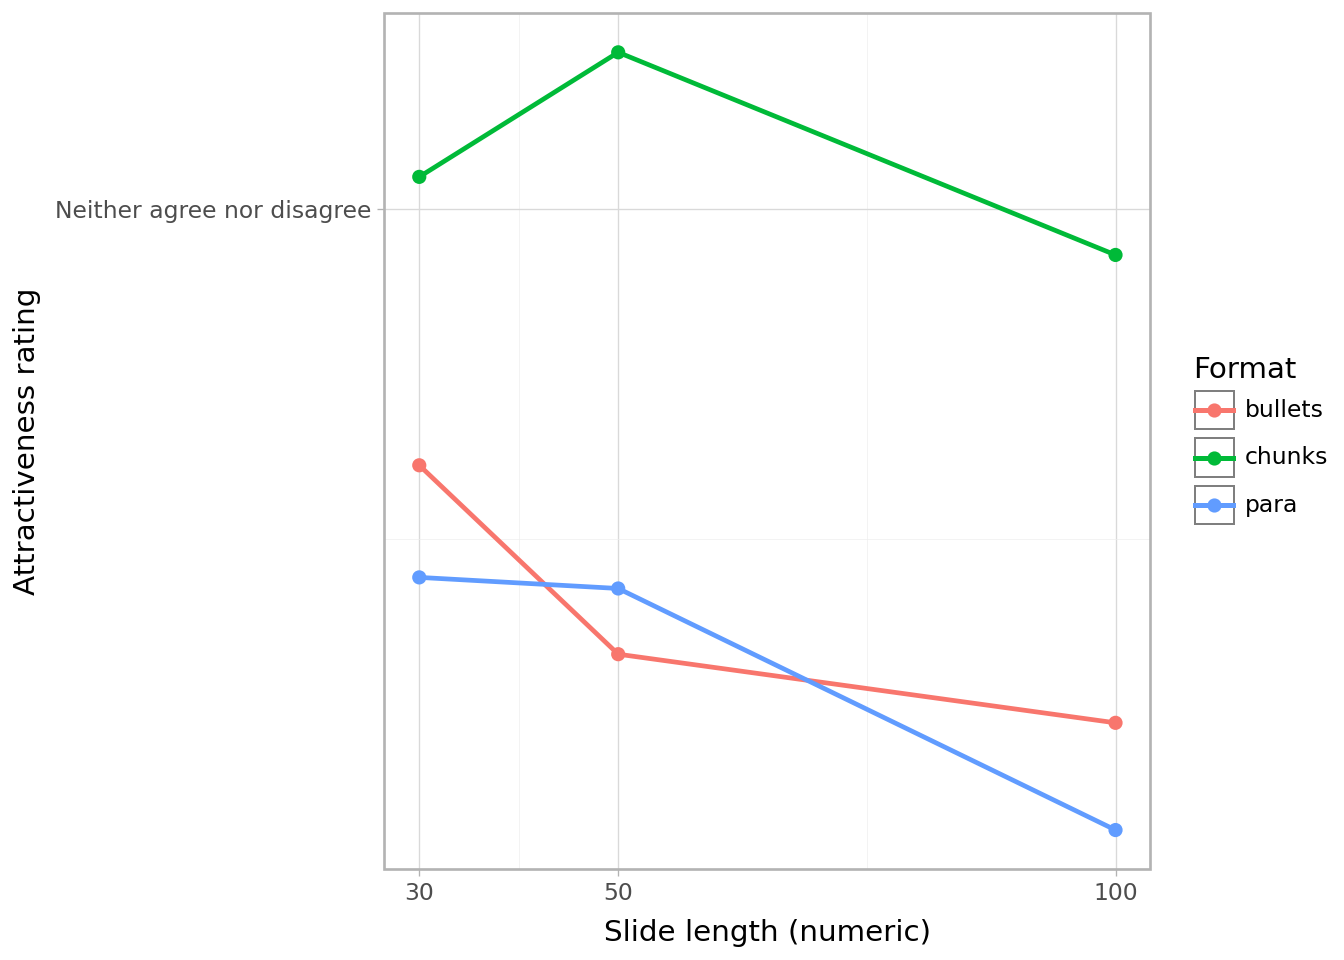
\includegraphics[width=7in,height=5in]{rieke-code_files/figure-pdf/cell-42-output-14.png}

\begin{tcolorbox}[enhanced jigsaw, arc=.35mm, bottomrule=.15mm, bottomtitle=1mm, breakable, colback=white, colbacktitle=quarto-callout-caution-color!10!white, colframe=quarto-callout-caution-color-frame, coltitle=black, left=2mm, leftrule=.75mm, opacityback=0, opacitybacktitle=0.6, rightrule=.15mm, title=\textcolor{quarto-callout-caution-color}{\faFire}\hspace{0.5em}{Caution}, titlerule=0mm, toprule=.15mm, toptitle=1mm]

This numeric trend plot treats slide length as a continuous predictor
and assumes a linear trend across 30, 50, and 100. In this study, slide
length was experimentally manipulated in discrete categories, so this
plot is best interpreted as a descriptive trend view rather than
definitive evidence of linearity.

\end{tcolorbox}

\begin{verbatim}
 
\end{verbatim}

\subsubsection{Cognitive load}\label{cognitive-load-1}

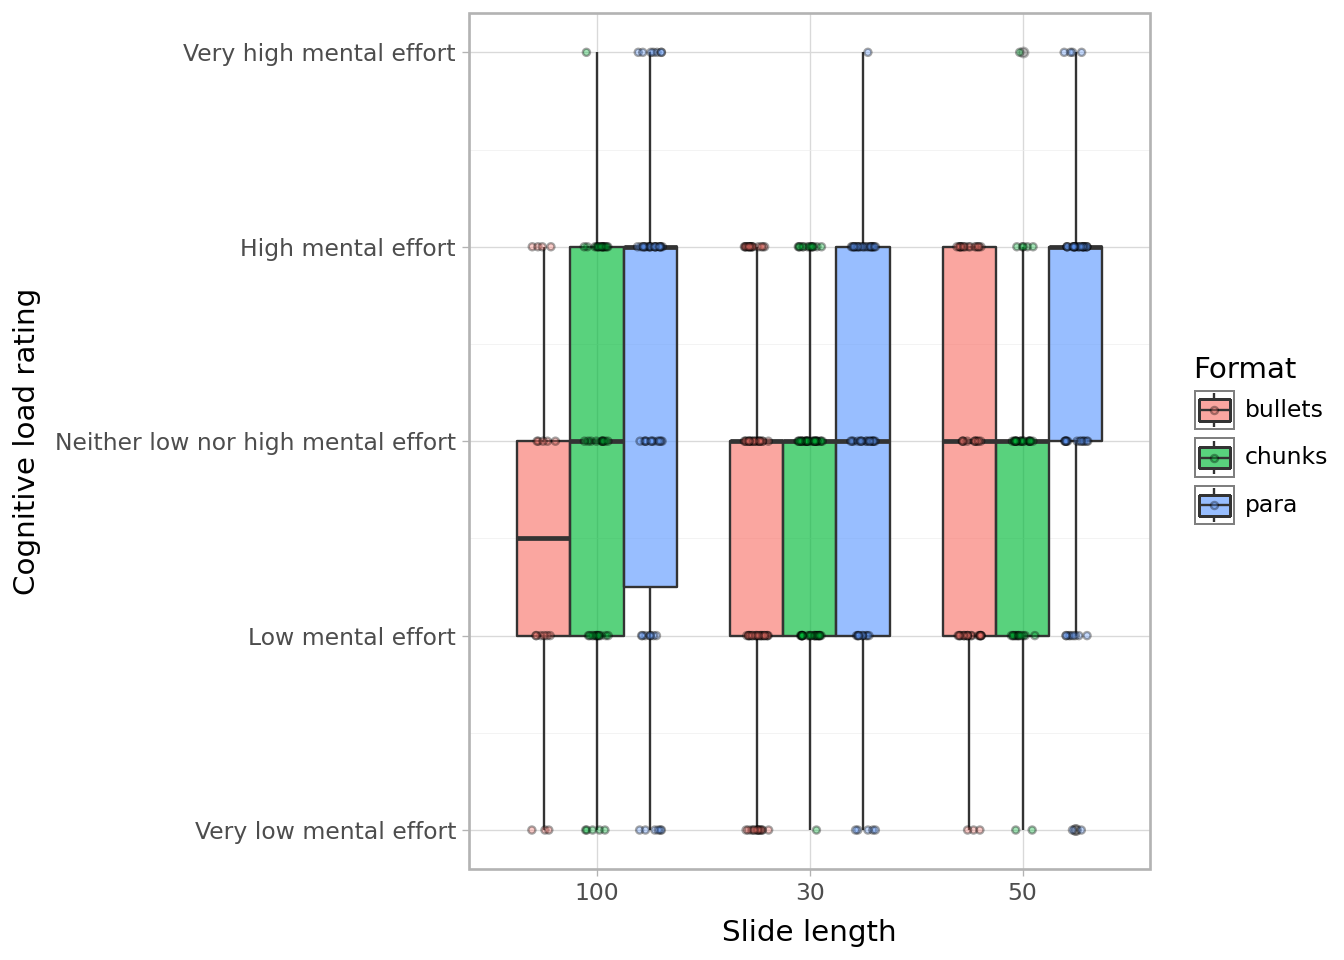
\includegraphics[width=7in,height=5in]{rieke-code_files/figure-pdf/cell-42-output-18.png}

\textbf{Main effects table}

{\def\LTcaptype{none} % do not increment counter
\begin{longtable}[]{@{}lrrl@{}}
\toprule\noalign{}
Effect & F & p\_value & Significant \\
\midrule\noalign{}
\endhead
\bottomrule\noalign{}
\endlastfoot
Slide length & 0.996259 & 0.370142 & No \\
Format & 11.4159 & 1.49287e-05 & Yes \\
Length x format & 0.499753 & 0.735941 & No \\
\end{longtable}
}

\textbf{No clear overall linear trend by slide length.}

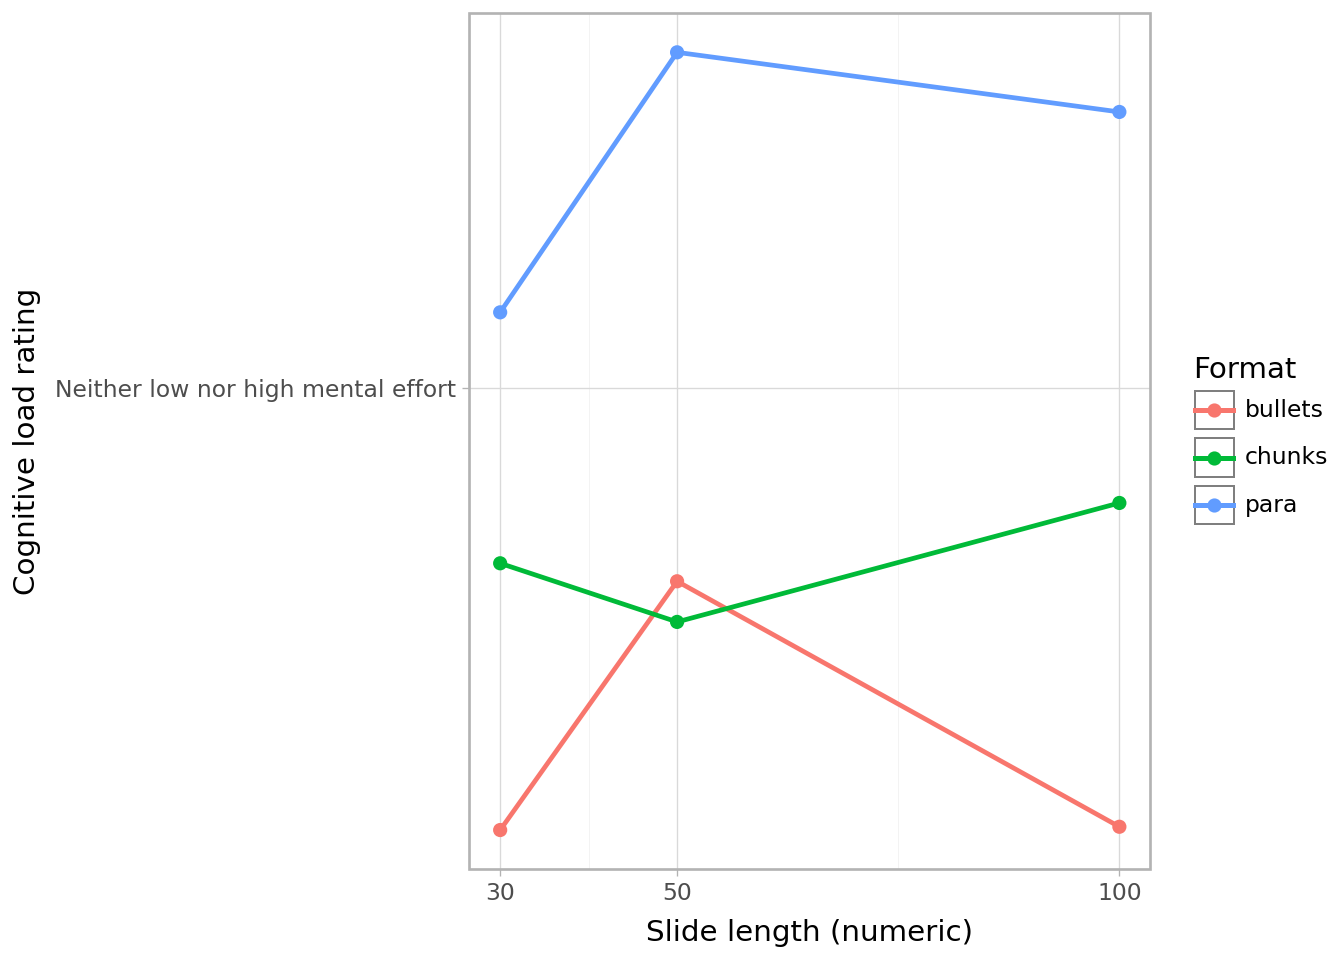
\includegraphics[width=7in,height=5in]{rieke-code_files/figure-pdf/cell-42-output-22.png}

\begin{tcolorbox}[enhanced jigsaw, arc=.35mm, bottomrule=.15mm, bottomtitle=1mm, breakable, colback=white, colbacktitle=quarto-callout-caution-color!10!white, colframe=quarto-callout-caution-color-frame, coltitle=black, left=2mm, leftrule=.75mm, opacityback=0, opacitybacktitle=0.6, rightrule=.15mm, title=\textcolor{quarto-callout-caution-color}{\faFire}\hspace{0.5em}{Caution}, titlerule=0mm, toprule=.15mm, toptitle=1mm]

This numeric trend plot treats slide length as a continuous predictor
and assumes a linear trend across 30, 50, and 100. In this study, slide
length was experimentally manipulated in discrete categories, so this
plot is best interpreted as a descriptive trend view rather than
definitive evidence of linearity.

\end{tcolorbox}

\begin{verbatim}
 
\end{verbatim}

\subsubsection{Slide simplicity}\label{slide-simplicity-1}

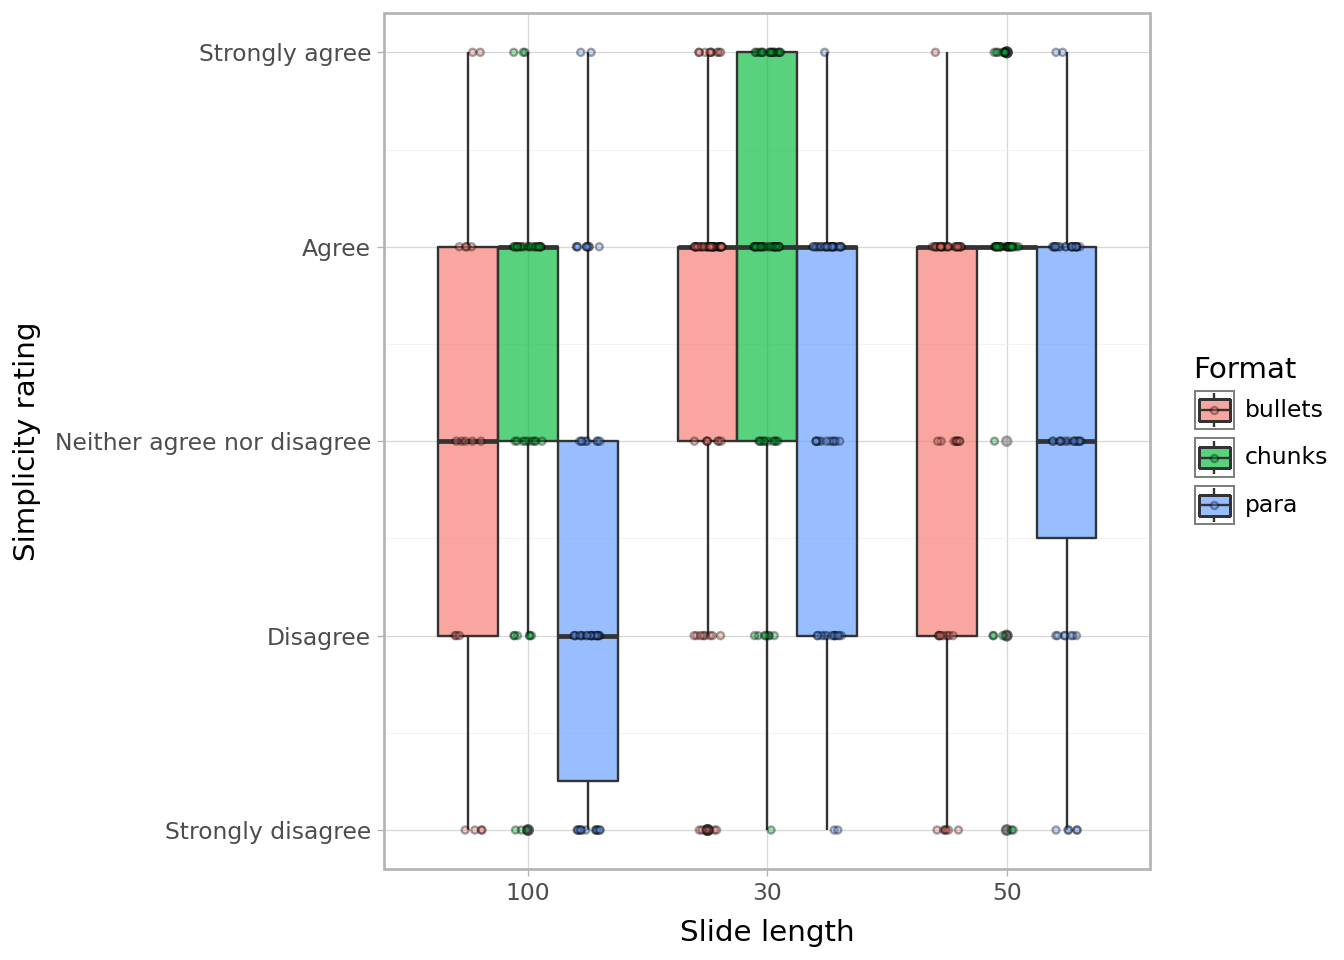
\includegraphics[width=7in,height=5in]{rieke-code_files/figure-pdf/cell-42-output-26.png}

\textbf{Main effects table}

{\def\LTcaptype{none} % do not increment counter
\begin{longtable}[]{@{}lrrl@{}}
\toprule\noalign{}
Effect & F & p\_value & Significant \\
\midrule\noalign{}
\endhead
\bottomrule\noalign{}
\endlastfoot
Slide length & 14.1038 & 1.18952e-06 & Yes \\
Format & 17.3776 & 5.68155e-08 & Yes \\
Length x format & 0.901128 & 0.463204 & No \\
\end{longtable}
}

\textbf{Overall, longer slides are rated as less simple and clean.}

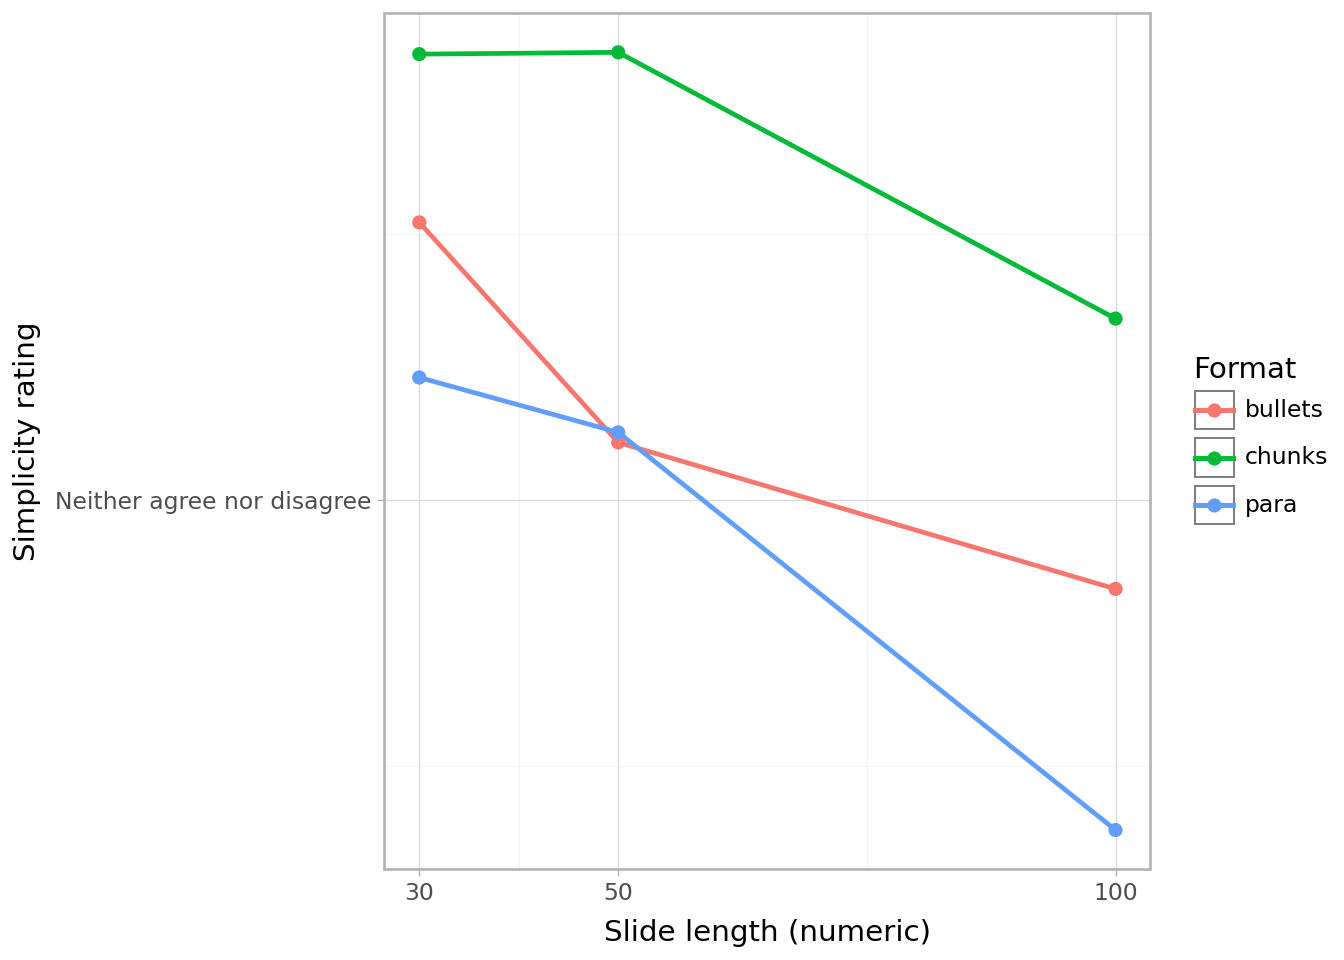
\includegraphics[width=7in,height=5in]{rieke-code_files/figure-pdf/cell-42-output-30.png}

\begin{tcolorbox}[enhanced jigsaw, arc=.35mm, bottomrule=.15mm, bottomtitle=1mm, breakable, colback=white, colbacktitle=quarto-callout-caution-color!10!white, colframe=quarto-callout-caution-color-frame, coltitle=black, left=2mm, leftrule=.75mm, opacityback=0, opacitybacktitle=0.6, rightrule=.15mm, title=\textcolor{quarto-callout-caution-color}{\faFire}\hspace{0.5em}{Caution}, titlerule=0mm, toprule=.15mm, toptitle=1mm]

This numeric trend plot treats slide length as a continuous predictor
and assumes a linear trend across 30, 50, and 100. In this study, slide
length was experimentally manipulated in discrete categories, so this
plot is best interpreted as a descriptive trend view rather than
definitive evidence of linearity.

\end{tcolorbox}

\begin{verbatim}
 
\end{verbatim}




\end{document}
